\documentclass[lang=cn, 10pt, titlestyle=display, oneside, toc=twocol]{elegantbook}
\usepackage{graphicx}
\usepackage{subfigure}
\usepackage{pgfplots}
\pgfplotsset{compat=1.18}
\usepackage{multicol}
\renewcommand{\theequation}{\Roman{equation}}
\tcbuselibrary{skins}
\usepackage{xcolor}
\usepackage{enumitem} % 提供 inline 列表
\usepackage{tikz}
\usetikzlibrary{arrows.meta}
\usepackage{etoolbox}
\usepackage{yhmath}
\usepackage{amsmath}  % 提供数学公式支持
\usepackage{array}    % 提供更强大的表格功能
\usepackage{wrapfig}
\setcounter{tocdepth}{2}
\usetikzlibrary{shapes,arrows}
\title{九年级数学讲义(人教版)}

\usepackage{xparse}
\usepackage{expl3} % 用于字符串处理
\tikzstyle{arrow} = [thick,->,>=stealth]
\hypersetup{
    colorlinks=true,
    linkcolor=blue,
    filecolor=blue,      
    urlcolor=blue,
    citecolor=cyan,
}

\newcommand{\exas}[2]{%
\begin{example}
#1
\begin{solution}
#2
\end{solution}
\end{example}
}

%%%%%%%%%%%%%%%%%%%%%%%%%%%%%%%%%%%%%%%%%%%%%%%%%%%%%%%%%%%%%%%%%%%%%%%%%%%%%%%%%%%%%
\begin{document}


\chapter*{前言}

\section*{使用}

电子版PDF点击目录跳转对应章节,跳转后对应章节的标题一般出现在页面最上方.打印自行删除前言.其他声明见后记




\tableofcontents



\chapter{一元二次方程}



%一元二次方程-基本
\input{QE_basics}
%配方
\section{配方}



配方是一种把二次多项式(如 \(ax^2 + bx + c\))通过添加和减去同一个项,转化为完全平方式的数学技巧.
\par
\begin{remark}
    完全平方是指一个数或代数式可以表示为另一个数或代数式的平方,例如\( 1=1^2,\ 4=2^2,\ \)(这些是数的完全平方)\(x^2+6x+9=(x+3)^2,\ 4x^2-12xy+9y^2=(2x-3y)^2\)等等.
\end{remark}
\par
在八年级我们学习过完全平方公式\(a^2+b^2\pm2ab=(a\pm b)^2\)来因式分解,这个公式本质上就是在配方. 但并不是所有式子都能使用这个公式来配方,例如\(x^2+2x\)就没有办法直接套用公式,面对这种情况就需要使用配方法来转化为一个有完全平方的式子,形如\(a(x+h)^2+k\),下面就用\(x^2+2x\)作为配方示范:
\begin{example}
给\(x^2+2x\)配方
\end{example}
\par
\begin{solution}
    \begin{enumerate}
  \item 分析一次项结构,将一次项分解为:\\
  \[
  2x = 2 \cdot x \cdot 1
  \]
  这对应完全平方公式中的 \(2ab\),其中 \(a = x\),\(b = 1\)
  
  确定需要添加的项,根据完全平方公式,需要添加 \(b^2\):
  \[
  b^2 = (1)^2 = 1
  \]
  
  \item 同时增减此项
  \begin{align*}
  x^2 + 2x &= x^2 + 2x + 1 - 1 \\
            &= (x^2 + 2x + 1) - 1
  \end{align*}
  
  \item 重组为完全平方式,前三项恰好是 \(x\) 和 \(1\) 的完全平方
  \begin{remark}
  将$1^2$移出括号不能忘记乘上括号前的系数1)
  \end{remark}
  \[
  = (x + 1)^2-1
  \]
  \item 一般来说最后需要整理方程,$(x + 1)^2-1$已经最简所以不用整理
\end{enumerate}

\end{solution}
以上是平方项(二次项)为1的情况,当平方项为1时,才能分解一次想的结构从而配出另一个平方项,但是当平方项不为1呢?这个时候就要先把平方项化为1,可以通过“因式分解-提取公因式”做到,下面以给\(2x^2 + 6x+1\)配方为例子
\par
%%%%%%%%%%%%%%%%%%%%%%%%%%%%%%%%%%%%%%%%%%%%%%%%%%%%%%%%%%%%%%%%%%%%%%%%%%%%%%
\begin{example}
    将 \(2x^2 + 6x+1\) 配方
\end{example}
\begin{solution}
\begin{enumerate}
    \item 提取前两项的系数 \(2\):
    \begin{align*}
    \text{原式} &= 2\left(x^2 + 3x\right) + 1
    \end{align*}

    \item 在括号内配方(补全平方):
    \begin{align*}
    &= 2\left[x^2 + 3x + \left(\frac{3}{2}\right)^2 - \left(\frac{3}{2}\right)^2\right] + 1\\
    &=2\left[\left(x + \frac{3}{2}\right)^2 - \frac{9}{4}\right] + 1
    \end{align*}

    \item 展开并合并常数项
    \begin{remark}
    将\(\frac{4}{9}\)移出括号不能忘记乘上提取的系数
    \end{remark}
    \begin{align*}
    &=2\left(x + \frac{3}{2}\right)^2 - \frac{9}{2} + 1 \\
    &= 2\left(x + \frac{3}{2}\right)^2 - \frac{7}{2}
    \end{align*}
\end{enumerate}

最终配方结果为:
\[
2\left(x + \frac{3}{2}\right)^2 - \frac{7}{2}
\]

\end{solution}

以上两道是已知一个平方项和一次项配另一个平方项的例题,你是否发现我们配的平方项和一次项系数之间的关系?
\par
当已知平方项的系数为1,设一次项系数为\(A\),那我们配上的项就是\((\dfrac{A}{2})^2\)(一次项系数的一半的平方),运用这个关系在配方时就不用再拆解一次项进行分析,但要注意必须在平方项系数为1时,所以在配方时先检查平方项系数是否为1,如果不是可以像例题1.6一样提取公因式把平方项系数化为1再配方,对于已知一个平方项和一次项配另一个平方项的题型,总结配方步骤如下:
\begin{enumerate}
    \item 把平方项(二次项)系数化为1
    \item 同时增加和减少一次项系数的一半的平方
    \item 将要配的三项写成完全平方形式(把要减去的项提出来时要乘上括号前的系数)
    \item 整理式子成一般形式:\( a(x + h)^2 + k \)
\end{enumerate}
\par
配方不仅能够因式分解,还可以解决一些其他的数学问题,例如配方得到多项式的极值,配方后开方降次解一元二次方程. 这一节先讲用配方得到式子的极值
\par
由于平方具有非负性,也就是说\(a^2\geq0\),且\(a=0\)时,\(a^2\)的最小值为0,根据这一点,
当二次多项式配方为 \( a(x + h)^2 + k \) 时,因为 \( (x + h)^2 \geq 0 \),所以:
\newline
\begin{itemize}[label=]
    \item 如果 \( a > 0 \),多项式的最小值为 \( k \)(当 \( x = -h \) 时取得);
    \item 如果 \( a < 0 \),多项式的最大值为 \( k \)(当 \( x = -h \) 时取得).
\end{itemize}

\begin{example}
若\(x\)为任意实数,求代数式\(x^2+4x+2\)的最小值
\end{example}

\begin{solution}

\begin{align*}
x^2 + 4x + 2 &= x^2 + 4x + 4 - 4 + 2 \\
&= (x^2 + 4x + 4) - 2 \\
&= (x + 2)^2 - 2.\\
\end{align*}
\begin{align*}
&\because (x + 2)^2 \geq 0\\
&\therefore (x + 2)^2-2 \geq -2\\
&\therefore x^2 + 4x + 2 \  \text{的最小值是}-2
\end{align*}
\end{solution}

\begin{exercise}
\small
    \setlength{\parindent}{0pt} % 取消段落缩进
    \setlength{\columnseprule}{0.01pt}
    \begin{multicols}{2}
        \begin{minipage}{1\linewidth}
        (1)给\( 4x^2 +1\)配上一个单项式,使之成为完全平方式.
        \end{minipage}
        
        \begin{minipage}{1\linewidth}
        (2)给下列多项式配方.
        \begin{enumerate}
            \item \((2x+1)^2-2(2x+1)+1\)
            \item \(3x^2-6x-2\)
            \item \(3x^2+8x-3\)
            \item \(x^2+2x+10\)
        \end{enumerate}
        \end{minipage}
%%%%%%%%%%%%%%%%%%%%%%%%%%%%%%%%%%%%%%%%%%%%%%%%%%%%%%%%%%%还有习题没编完,参考5星学霸第六页
        \begin{minipage}{1\linewidth}
        (3)\(-x^2+4x-7\)的最小值是\underline{\hspace{3.5em}},此时\(x=\)\underline{\hspace{3.5em}}
        \end{minipage}

        \begin{minipage}{1\linewidth}
        (4)若\(W=5x^2-4xy+y^2-2y+8x+3(x,y\text{为实数}),\text{则}W\)的最小值为\underline{\hspace{3.5em}}
        \end{minipage}

        (5)已知\(M=x^2+2y^2, N=2xy+y-m\),当\(M>N\)恒成立时,求\(m\)的取值范围.
        
    \end{multicols}
\end{exercise}



%配方的意义重大->如何配方->配方看取值->配方分解因式

%配方法解方程->用配方发推导出公式法->根的判别式->求根公式解方程->因式分解



%解一元二次方程
\section{解一元二次方程}
1.1学习了关于一元二次方程的基本内容包括一元二次方程的定义和判定,将一元二次方程转化为一般形式的能力,之后的小节与前面的知识点是强关联的,所以请及时温习知识仔细做题. 1.2主要学习了如何给二次多项式配方和用配方得到式子的极值,前面提到过运用配方可以解一元二次方程,具体来说是将方程配方后等式两边同时开方达到\textbf{降次}的目的
\par
在初中,解高次方程的主要思路是降次,降次是指通过数学变形(如因式分解、换元、展开等)将一个高次问题转化为低次问题(例如把一元二次方程问题转变为一元一次方程的问题),从而简化计算或求解过程,在初中常用的降次方法有配方后开方降次、因式分解降次、展开消元降次、求根公式降次等,本节主要学习用不同方法达到降次的目的,灵活使用不同的方法降次解方程是练习的重点.
\subsection{配方法(配方后开方降次)}


\par


配方法的基本思路是将方程式配方,再将两边同时开方降次,将一元二次方程问题转化为一元一次方程问题是配方法的内容.

\begin{example}
    用配方法解关于\(x\)的方程\((2x+4)x - 1 = 0\)
\end{example}
\begin{solution}
\noindent
\[
\begin{aligned}
&\text{1. 将方程转化为一般形式:} && 2x^2 + 4x - 1 = 0 \quad\Rightarrow\quad 2x^2 + 4x = 1 \\[2pt]
&\text{2. 配方:} && 2\left(x^2 + 2x\right) = 1 \quad\Rightarrow\quad 2\big[(x+1)^2 - 1\big] = 1 \\[2pt]
&\text{3. 展开整理:} && 2(x+1)^2 - 2 = 1 \quad\Rightarrow\quad (x+1)^2 = \frac{3}{2} \\[2pt]
&\text{4. 开平方:} && |x+1| = \frac{\sqrt{6}}{2} \quad\Rightarrow\quad x+1 = \pm\frac{\sqrt{6}}{2} \\[2pt]
&\text{5. 解 \(x\):} && x = -1 \pm \frac{\sqrt{6}}{2} \quad\Rightarrow\quad x_1 = -1 + \frac{\sqrt{6}}{2},\ x_2 = -1 - \frac{\sqrt{6}}{2}
\end{aligned}
\]




\end{solution}
通过这道例题,我们可以得出使用配方法解一元二次方程的步骤,步骤看似很多实际上在1.2经过充分练习后你应该能熟练掌握配方的步骤:
\begin{enumerate}
    \item 整理为一般形式,常数项移到等式右边
    \item 配方
        \begin{enumerate}
        \item 把平方项(二次项)系数化为1
        \item 同时增加和减少一次项系数的一半的平方
        \item 将要配的三项写成完全平方形式
        \item 整理方程成\((x + n)^2=p\)的形式
        \end{enumerate}
    \item \textbf{判断根的情况}(见下文和例题1.9)
    \item 开方降次(\(p\ge0\))
\end{enumerate}
\par
\begin{remark}
    不能把配方和解一元二次方程时使用配方法(配方后开方降次)混为一谈
\end{remark}
在例题1.8中第3步将方程整理成了\((x + n)^2=p\)的形式,这时要方程两边同时开平方就要考虑\(p\)的取值,我们可以通过\((x + n)^2=p\)进行推导得出不同的情况:
\begin{enumerate}
    \item 当\(p>0\)时,
    \begin{align*}
        \sqrt{(x + n)^2}&=\sqrt{p}\\
        |x+n|&=\sqrt{p}\\
        x&=-n\pm\sqrt{p}\\
        x_1=-n + \sqrt{p},\ x_2&=-n - \sqrt{p}\\
    \end{align*}
    $\therefore \text{有两个不相等的实数根}$
    \item 当\(p=0\)时,
    \begin{align*}
        \sqrt{(x + n)^2}&=\sqrt{0}\\
        |x+n|&=0\\
        x&=-n\\
        x_1=x_2&=-n\\
    \end{align*}
    $\therefore \text{有两个不相等的实数根即重根}$
    \item 当\(p<0\)时,因为对于任何实数\(x\),都有\((x+n)^2\ge0\)而\(p<0\),所以无实数根.

\end{enumerate}
根据上面的推导,我们就能够判断根的情况当(\(p\ge0\))时开方降次,在\(p<0\)时直接写“原方程无实数根”即可,下面以\( x^2 - 6x = -9 \)和\( x^2 + 4x + 5 = 0 \)为例:
\par
\begin{example}
    解关于\(x\)的一元二次方程:(1)\( x^2 - 6x = -9 \),(2)\( x^2 + 4x + 5 = 0 \)
\end{example}

\begin{solution}
    \begin{multicols}{2}
    \begin{minipage}{1\linewidth}
        (1)
        \begin{align*}
        x^2 - 6x + \left(\frac{-6}{2}\right)^2 &= -9 + \left(\frac{-6}{2}\right)^2 \\
        x^2 - 6x + 9 &= -9 + 9 \\
        (x - 3)^2 &= 0 \\
        x &= 3 \\
        x_1=x_2 &= 3
        \end{align*}\\
    \end{minipage}
    \begin{minipage}{1\linewidth}
        (2)
        \begin{align*}
        x^2 + 4x &= -5 \\
        x^2 + 4x + \left(\frac{4}{2}\right)^2 &= -5 + \left(\frac{4}{2}\right)^2 \\
        x^2 + 4x + 4 &= -5 + 4 \\
        (x + 2)^2 &= -1 \\
        \therefore \text{原方程无实数根}
        \end{align*}
    \end{minipage}
    \end{multicols}
\end{solution}
%theorem、lemma、corollary、axiom、postulate
\begin{exercise}
\small
    \setlength{\parindent}{0pt} % 取消段落缩进
    \setlength{\columnseprule}{0.01pt}
    \begin{multicols}{2}
        用配方法解下列方程\\
        (1)\(x^2+4x+4=0\)\\
        (2)\(x^2-6x+7\)\\
        (3)\(3x^2-12x=-12\)\\
        (4)\(2x^2+4x-5=0\)\\
        (5)\(2x^2-3x+1=0\)\\
        (6)\(2x^2-6x-9=0\)\\
        (7)\(2x^2-7x=2\)\\
        (8)\(x(x-4)=2-8x\)\\
        (9)\(x^2+5x+3\)\\
    \end{multicols}
\end{exercise}



\subsection{求根公式法}


使用配方法解一元二次方程的核心思想是通过配方使方程得到形似\((x+n)^2=p\)的形式,因为等式两边都是完全平方式,所以可以同时开平方降次,但是这样的做法比较繁琐,于是我们就将配方法法用在一元二次方程的一般形式上得到一个通用的求一元二次方程的根的公式,我们称它为求根公式.
\begin{theorem}[一元二次方程求根公式]
对于任意一元二次方程 $ax^2 + bx + c = 0$($a \neq 0$),其解为:
\[
x = \frac{-b \pm \sqrt{b^2 - 4ac}}{2a}
\]
其中 $b^2 - 4ac$ 称为判别式($\Delta$),根的性质取决于判别式的值:
\begin{itemize}
    \item 当 $\Delta > 0$ 时,方程有两个不相等的实数根;
    \item 当 $\Delta = 0$ 时,方程有两个相等的实数根(重根);
    \item 当 $\Delta < 0$ 时,方程有一对共轭复数根。
\end{itemize}
\end{theorem}

\begin{proof}
通过配方法推导如下:
\begin{align*}
    x^2 + \frac{b}{a}x + \frac{c}{a} &= 0\\
    x^2 + \frac{b}{a}x &= -\frac{c}{a}\\
    x^2 + \frac{b}{a}x + \left(\frac{b}{2a}\right)^2 &= -\frac{c}{a} + \left(\frac{b}{2a}\right)^2 \quad \text{(配方)} \\
    \left(x + \frac{b}{2a}\right)^2 &= \frac{b^2}{4a^2} - \frac{c}{a}\\
    \left(x + \frac{b}{2a}\right)^2 &= \frac{b^2 - 4ac}{4a^2}\\
    %|x + \frac{b}{2a}| &= \frac{\sqrt{b^2 - 4ac}}{2a}
\end{align*}
\end{proof}
因为\(a\ne0\),所以\(4a^2>0\)保证了分母不为0可以继续计算,但在开方降次之前,发现判别式\(b^2 - 4ac\)的值会影响到根的情况(如果$b^2 - 4ac<0$ 则不能开方,因为就我们目前的知识无法解决根号下是负数的开方计算,因此需要分别讨论判别式的取值情况.
\begin{enumerate}
    \item 当\(b^2 - 4ac>0\)时,
    \begin{align*}
        x_1 = \frac{-b + \sqrt{b^2 - 4ac}}{2a}, \quad x_2 = \frac{-b - \sqrt{b^2 - 4ac}}{2a}\\
    \end{align*}
    $\therefore \text{有两个不相等的实数根}$
    \item 当\(b^2 - 4ac=0\)时,
    \begin{align*}
         x &= \frac{-b \pm 0}{2a}\\
    &= -\frac{b}{2a}\\
    \end{align*}
    $\therefore \text{有两个不相等的实数根即重根}$
    \item 当\(b^2 - 4ac<0\)时,因为\(b^2 - 4ac<0\)此时\(\dfrac{b^2 - 4ac}{4a^2}<0\),相当于\((x + \dfrac{b}{2a})^2<0\),此时\(x\)取任何实数都不能使得\((x + \dfrac{b}{2a})^2<0\),所以原方程无实数根.

\end{enumerate}
\par
我们称\(b^2 - 4ac\)为判别式\(\Delta\),判别式的主要作用是判断根的情况(三种情况是有两个不相等的实数根、有两个相等的实数根和无实数根)
\par
\begin{remark}
注意与之前的知识做区分:前面提到过 一元二次方程一般形式中\(a\ne0\)的作用是保证方程未知数的最高次数为2(保证方程是二次方程),而这里的判别式是用于判断方程的根的情况,不要混淆使用. 
\end{remark}
\par
如果我们知道方程的系数就可以使用判别式推导出根的情况,如果我们知道根的情况和部分系数通过判别式我们可以推导出方程中其他的系数.
\begin{example}
    已知关于\(x\)的一元二次方程\(x^2+2mx+m^2+m-2=0\)有实数根.求\(m\)的取值范围
\end{example}
\begin{solution}
(1)分析:阅读题目,题目告诉我们该方程有实数根,因此\(\Delta\ge0\),因为\(m\)是该方程的一个参数在部分系数之中,所以我们可以通过求判别式的再列关于\(m\)的不等式得出\(m\)的取值范围. \textbf{先逐个列出该方程的系数},然后代入判别式,由\(\Delta\ge0\)列不等式,最后求出\(m\)的取值范围
\begin{align*}
    \because& a=1,\ b=2m,\ c=m^2+m-2\\
    \therefore& \Delta = b^2-4ac=(2m)^2-4\times1\times(m^2+m-2)=-4m+8\\
    \because& \Delta>0\\
    \therefore& -4m+8>0\\
    \therefore& 解得m\le2
\end{align*}
\end{solution}
\small
\par
由于判别式值的不同导致了\(x\)的结果不同,所以在每次使用求根公式解一元二次方程的时候都需要先计算判别式的值,再代入不同情况的公式,一般习惯先把系数列出来再代入判别式不易出错,下面通过例题学习使用求根公式解方程的过程
\begin{example}
    用公式法解方程:(1)\( 2x^2 - 4x + 2 = 0 \),(2)\( x^2 + 2x + 3 = 0 \) (3)\( 2x^2 - 5x + 2 = 0 \)
\end{example}
\begin{solution}
\vspace{-0.8cm}
\begin{multicols}{3}
\begin{enumerate}
\vspace{-0.5cm}
    \item \begin{align*}
&\text{1. 确定系数:}\\
&a = 2,\ b = -4,\ c = 2. \\
&\text{2. 计算判别式:}\\
\Delta &= b^2 - 4ac\\
&= (-4)^2 - 4 \times 2 \times 2\\
&= 16 - 16\\
&= 0. \\
&\text{3. 代入求根公式:}\\
&x = -\frac{b}{2a} = -\frac{-4}{4} = \frac{4}{4}. \\
&\text{4. 求得重根:}\\
&x_1=x_2 = 1.
\end{align*}
    \item \begin{align*}
a &= 1, \quad b = 2, \quad c = 2, \\
\Delta &= b^2 - 4ac \\
  &= (2)^2 - 4 \times 1 \times 2 \\
  &= 4 - 8 \\
  &= -4.\\
&\because \Delta<0\\
&\therefore \text{原方程无实数根}
\end{align*}
    \item \begin{align*}
a &= 2, \quad b = -5, \quad c = 2, \\
\Delta &= b^2 - 4ac \\
  &= (-5)^2 - 4 \times 2 \times 2 \\
  &= 25 - 16 \\
  &= 9, \\
x &= \frac{-b \pm \sqrt{b^2 - 4ac}}{2a} \\
  &= \frac{-(-5) \pm \sqrt{9}}{2 \times 2} \\
  &= \frac{5 \pm 3}{4}, \\
x_1 &= \frac{5 + 3}{4} = 2, \ 
x_2 = \frac{5 - 3}{4} = \frac{1}{2}.
\end{align*}
\end{enumerate}
\end{multicols}

\end{solution}

通过例题,得出使用求根公式解一元二次方程的步骤:
\begin{enumerate}
    \item 列出二次项系数、一次项系数、常数项
    \item 计算判别式的值判断根的情况
    \item 使用对应公式
\end{enumerate}
\par
解高次方程的基本思路是降次,在用求根公式解方程时虽然没有体现降次这个步骤,但求根公式由配方法推导而来,降次步骤已经包含其中.
\begin{exercise}
\setlength{\parindent}{0pt} % 取消段落缩进
\setlength{\columnseprule}{0.01pt}
\begin{multicols}{2}
    (1)用公式法解下列方程:
    \begin{enumerate}
        \item \(3x^2-2x-2=0\)
        \item \(\dfrac{1}{2}x^2-5x+4=0\)
        \item \(2x^2-3(x+1)=0\)
        \item \((x+3)(x-1)=3\)
    \end{enumerate}
    (2)已知关于\(x\)的一元二次方程方程\(x^2-(m+2)x+2m=0\).\\
    1.求证:无论\(m\)取任何实数,方程总有实数根\\
    2.若等腰三角形的一边长为3,另外两边长恰好是这个方程的两个根,求\(m\)的值.
\end{multicols}
\end{exercise}

\subsection{因式分解法}

\begin{property}
    零因子法则:如果两个因式的乘积是0,则这两个因式至少有一个等于0;反之,如果两个因式中任意一个为0,他们的乘积为0
\end{property}

根据这一性质,假设有关于\(x\)的一元二次方程\((x+1)(x-1)=0\)则\((x+1),(x-1)\)之中至少有一个为0,那么令这两个因式分别为0就可以得到两个一元一次方程,将二次问题转化为了一次问题,达到了降次的目的,只需要分别分别解出两个一次方程就可以得到方程的根,以下是过程:
\begin{align*}
    (x+1)(x-1)=0
\end{align*}
\begin{solution}
    \begin{align*}
        x+1=0, x-1=0\\
        解得x_1=-1,x_2=1\\
    \end{align*}
\end{solution}
相较于前面的方法,使用零因子法则降次的过程更加简洁,但是你是否注意到了,前面在学习配方法解一元二次方程的时候我们提到过,我们将方程化为\((x+n)^2=p\)的形式后降次,此时p的值会影响根的情况,在学习用求根公式解方程的时候,我们使用判别式判断根的情况,但在这里似乎省略了判断根的情况?表面上看来确实是这样,不需要判断根的情况是使用因式分解法的优势也是它的过程更简洁的原因,那么根的情况又由什么决定呢?
\par
实际上根的情况由这两个因式决定,假设有关于\(x\)的方程\((x+m)(x+n)\),如果两个因式化成的两个方程的解都在实数范围内,实际上这个方程就有两个实数根,如果\(m=n\)或者一个解不在实数范围内另一个解在实数范围内,原方程有两个相等的实数根,如果两个解都不在实数范围内,也就是说原方程无实数根. 这段话理解即可,在实际做题中我们要发挥因式分解法最大的优势就是在解题过程中不用思考根的情况.

在八年级我们学习过用提公因式(提取式子中的最大公因式)和乘法公式(平方差公式或完全平方公式)来因式分解,因式分解是指将一个多项式表示为若干个不可约多项式的乘积形式的过程
\par
实际上一元二次方程可以理解为是一个多项式方程,所以我们也可以对一元二次方程进行因式分解,得到形似\((x+m)(x-n)=0\)的结构,再运用零因子法则,分别得到两个方程,直接解即可得到答案:

\begin{enumerate}
    \item 对方程因式分解
    \item 拆解成两个方程,直接计算出结果
\end{enumerate}



%%%%%%%%%%%%%%%%%%%%%%%%%%%%%%%%%%%%%%%%%%%%%%%%%%%%%%%%%%%%%%%%%%%%%%%%%%%未完工,十字相乘法
\begin{example}
    用因式分解法解方程:(1) \((x-3)^2-49=0\). (2) \((5x-3)^2+2(3-5x)=0\).
\end{example}

\begin{solution}
\begin{multicols}{2}
(1) \((x-3)^2-49=0\):
\begin{align*}
(x-3)^2 - 49 &= 0 \\
(x-3)^2 &= 49 \\
x-3 &= \pm 7 \\
x &= 3 \pm 7, \\
x_1 &= 3 + 7 = 10, \\
x_2 &= 3 - 7 = -4.
\end{align*}

(2) \((5x-3)^2+2(2-5x)=0\):
\begin{align*}
(5x-3)^2 + 2(3-5x) &= 0 \\
(5x-3)^2 - 2(5x-3) &= 0 \\
(5x-3)\left[(5x-3) - 2\right] &= 0 \\
(5x-3)(5x-5) &= 0 \\
5x-3 = 0 \quad &\text{或} \quad 5x-5 = 0, \\
x_1 &= \frac{3}{5}, \\
x_2 &= 1.
\end{align*}
\end{multicols}
\end{solution}

设二次三项式为 $ax^2 + bx + c$,若能分解为 $(px + q)(rx + s)$,则需满足:
\begin{align*}
pr = a,
qs = c,ps + qr = b
\end{align*}
该方法通过交叉相乘验证系数的匹配关系,称为十字相乘法.
\par
并不是所有一元二次方程都可以使用十字相乘法因式分解,这时候就要灵活使用其他方法解方程.

%韦达定理(根与系数的关系)
\input{QE_Vietas_formulas}
%一元二次方程的根
\input{QE_root}
%一元二次方程与实际问题
\input{QE_practical_problems}

\section{有关一元二次方程的新定义}


%%%%%%%%%%%%%%%%%%%%%%%%%%%%%%%%%%%%%%%%%%%%%%%%%%%%%%%%%%%%%%%%%%%%%%%%%%%%%%%%%%%%%%%%%%%%%%%%%%%%%%%%%%%%%%%%%%%%%%%%%%%%%%%%%%%%%%%%%%%%%%%%%%%%%%%%%%%%%%%%%%%%%%%%%%%%%%%%%%%%%%%%%%%%%%%%%%%%%%%%%%%%%%%%%%%%%%%%%%%%%%%%%%%%

\chapter{二次函数}
%二次函数基本
\section{二次函数的基本}

在八年级学习过函数的定义:一般地,在一个变化过程中,如果有两个变量\(x\)与\(y\),并且对于\(x\)的每一个确定的值,\(y\)都有唯一确定的值与之对应,那么我们就说\(x\)是自变量,\(y\)是\(x\)的函数.
\par
当自变量\(x\)和因变量\(y\)有如下关系:
\(y=kx+b\)
则此时称\(y\)是\(x\)的一次函数. 特别地,当\(b=0\)时,\(y\)是\(x\)的正比例函数.
\par
本章学习另一种函数:二次函数. 首先从二次函数的基本性质入手,再运用性质解决不同的问题,学习本章不仅需要熟悉基本的知识,还要积累经验和技巧.


\subsection{二次函数的定义}

\begin{definition}
一般地,形如\(y=ax^2+bx+c\)(\(a,\ b,\ c\)是常数,\(a\ne0\))的函数, 叫做二次函数.
\par
其中\(x\)是自变量,\(y\)是\(x\)的函数,\(a,\ b,\ c\)分别表示函数解析式的二次项系数、一次项系数、常数项.
\end{definition}

根据课本的定义,可以得到二次函数必须具有的条件:
\begin{enumerate}
    \item 关系式为整式
    \item 自变量最高次数为2(注意系数\(a\ne0\)保证二次项存在)
\end{enumerate}

\subsection{二次函数的图像}

先描点,再用平滑的线连接,就能得到这个二次函数的图像

%%%%%%%%%%%示例函数图像%%%%%%%%%%%%%%%%%%%%%%%%%%%%%%%%%%%%%%%%%%%%%%%%%%%%%%%%%%%%%%%%%%%%%%%%%%%%%%%%%%%%%%%%%%%%%%%%%%%%%%%%%%%%%%%%%%%%%%%%%%%%%%%%%%%%%%%%%%%%%%%%%

\begin{table}[h]
\centering
\renewcommand{\arraystretch}{1.2} % 增加行高
\begin{tabular}{|c|*{7}{c|}} \hline
\( x \) & \(-3\) & \(-2\) & \(-1\) & \(0\) & \(1\) & \(2\) & \(3\) \\ \hline\hline
\( y \) & \(9\) & \(4\) & \(1\) & \(0\) & \(1\) & \(4\) & \(9\) \\ \hline
\end{tabular}
\caption{\( y = x^2 \) 的函数值表}
\end{table}

\begin{figure}[h]
    \centering
    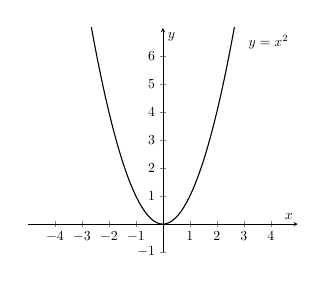
\begin{tikzpicture}[scale=0.5]
    \begin{axis}[
        axis lines = middle,       % 坐标轴居中
        > = Stealth,
        xlabel = $x$,             % x轴标签
        ylabel = $y$,             % y轴标签
        xmin = -5, xmax = 5,      % x轴范围
        ymin = -1, ymax = 7,      % y轴范围
        xtick = {-4,-3,...,4},    % x轴刻度
        ytick = {-1,...,1,2,3,4,5,6},  % y轴刻度
        legend pos = north west,  % 图例位置
    ]
    
    \addplot [
        domain = -5:6,
        samples = 100,
        thick
    ] {x^2};
    
    \node[anchor=west] at (axis cs:3,6.5) {\(y=x^2\)};
    
    \end{axis}
    \end{tikzpicture}
    \caption{}
    \label{fuc_1}
\end{figure}

类似的,按照步骤能画出不同的函数图像.
\par
通过图像可以看出二次函数\(y=x^2\)的图像是一条抛物线,实际上所有的二次函数图像都是抛物线\footnote{伽利略(Galileo Galilei)(1564-1642)通过实验发现抛射体运动轨迹是抛物线,将物理现象与二次函数图像明确对应,笛卡尔(René Descartes)(1596-1650)创立解析几何(1637年《几何学》)首次用坐标系证明抛物线对应\(y=ax²+bx+c\)形式的方程.},所以我们把二次函数\(y=ax^2+bx+c\)的图像也叫做抛物线\(y=ax^2+bx+c\).
\par
观察图\ref{fuc_1}还能发现二次函数\(y=x^2\)是一个轴对称图形,而\(x=0\)则是他的对称轴,实际上所有二次函数都是轴对称图形,所有二次函数都有它的\textbf{对称轴},而\textbf{二次函数与对称轴的交点}称为二次函数的\textbf{顶点},在图\ref{fuc_1}中,抛物线\(y=x^2\)的顶点是\((0,0)\),也就是原点.
\par
图\ref{fuc_1}中\(x\)和\(y\)的关系,在抛物线的左侧也就是\(x>1\)时,\(y\)随\(x\)的增大而增大,当\(x<1\)时,\(y\)随\(x\)的增大而减小.函数在某一范围内随着自变量的增大而减小的性质可以取名为增减性\footnote{在未来的学习中,会更加准确的了解这个性质的定义,在高中教材称为单调性}.
\par
现在的抛物线$y=x^2$中,二次项系数的值为1,如果改变二次项系数$a$图像会发生变化吗?如果用作\(y=\dfrac{1}{2}x,y=-x^2, y=-\dfrac{1}{2}x^2\)三个函数的图,得出当\(a>0\)时,抛物线的开口向上,当$a<0$时,抛物线的开口向下,\(a\)的绝对值($|a|$)越大,开口越小,$|a|$越小开口越大

\begin{conclusion}
总结性质如下:
\begin{enumerate}
    \item 二次函数的图像是\textbf{轴对称图形},并且有唯一的一条\textbf{对称轴}.  
          对称轴与抛物线的交点称为\textbf{顶点},例如 \(y = x^2\) 的顶点是 \((0, 0)\).
    \item 对于二次函数 \(y = ax^2 + bx + c\),当自变量 \(x\) 在不同区间变化时,函数值会呈现\textbf{增减性}: 
    \begin{enumerate}
              \item 在顶点左侧,\(y\) 随 \(x\) 的增大而减小;  
              \item 在顶点右侧,\(y\) 随 \(x\) 的增大而增大.
          \end{enumerate}
    \item 二次项系数 \(a\) 对抛物线形状的影响:  
          \begin{enumerate}
              \item 当 \(a > 0\) 时,抛物线开口向上;  
              \item 当 \(a < 0\) 时,抛物线开口向下;  
              \item \(|a|\) 越大,抛物线开口越窄;  
              \item \(|a|\) 越小,抛物线开口越宽.
          \end{enumerate}
\end{enumerate}
\end{conclusion}


%%%%%%%%%%%%%%%%%%%%%%%%%%接例题图像性质

\begin{wrapfigure}{r}{3cm}
\vspace{-1cm}
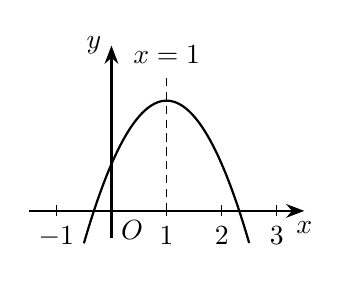
\begin{tikzpicture}[scale=0.7, >=Stealth, declare function={f(\x) = -1.15*(\x-1)^2 + 2;}]
                                            % 坐标轴设置
                                            \draw[->, thick] (-1.5,0) -- (3.5,0) node[below] {$x$}; % x轴
                                            \draw[->, thick] (0,-0.5) -- (0,3) node[left] {$y$}; % y轴 (高度4cm)
                                            
                                            % 横轴刻度 (范围-1~3,不显示0)
                                            \foreach \x in {-1,1,2,3} {
                                                \draw (\x,0.1) -- (\x,-0.1) node[below] {$\x$};
                                            }
                                            
                                            % 原点标记为O
                                            \draw (0,0) node[below right] {$O$};
                                            
                                            % 对称轴 (x=1 虚线)
                                            \draw[densely dashed] (1,0) -- (1,2.5) node[above] {$x=1$};
                                            
                                            % 绘制二次函数 (开口向下)
                                            \draw[thick, domain=-0.5:2.5, samples=100] plot (\x, {f(\x)});
                                            
                                            \end{tikzpicture}
                                            \caption{}
                                            \label{b1}
\end{wrapfigure}


\exas{
如图\ref{b1},已知二次函数\(y=ax^2+bx+c\ (a\ne0)\)的图像如下,有下列5个结论:
\begin{enumerate*}[label=\textcircled{\arabic*}, itemjoin={;}]
    \item \(abc > 0\)
    \item \(4a+2b+c > 0\)
    \item \((a+c)^2> b^2\)
    \item \(2c>3b\)
    \item \(a+b>m(am+b)\)(\( m\ne 1\)的实数)
\end{enumerate*}
. 其中正确的有(\hspace{3em})
\par
\begin{enumerate*}[label=\Alph*., itemjoin={\hspace{3em}}]
    \item 1个
    \item 2个
    \item 3个
    \item 4个
\end{enumerate*}
}{}
%%%%%%%%%%%%%%%%%%%%%%%%%%%%%%%%%%%%%%%%%%%%%%%%%%%%
\begin{wrapfigure}{r}{3cm}
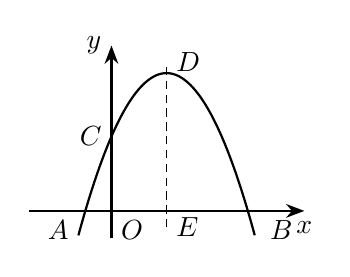
\begin{tikzpicture}[scale=0.7, >=Stealth, 
                                                    declare function={f(\x) = -1.15*(\x-1)^2 + 2.5;}] % 调整抛物线形状
                                                
                                                % 坐标轴设置
                                                \draw[->, thick] (-1.5,0) -- (3.5,0) node[below] {$x$}; % x轴
                                                \draw[->, thick] (0,-0.5) -- (0,3) node[left] {$y$}; % y轴
                                                
                                                % 原点标记
                                                \draw (0,0) node[below right] {$O$};
                                                
                                                % 对称轴 (x=1 虚线)
                                                \draw[densely dashed] (1,-0.3) node[right] {$E$} -- (1,2.7) node[right] {$D$};
                                                
                                                % 关键点标注
                                                \filldraw (-0.6,0) circle (0pt) node[below left] {$A$};
                                                \filldraw (2.7,0) circle (0pt) node[below right] {$B$};
                                                \filldraw (0,1.35) circle (0pt) node[left] {$C$}; % C点y坐标由f(0)计算
                                                
                                                % 绘制抛物线
                                                \draw[thick, domain=-0.6:2.6, samples=100] plot (\x, {f(\x)});
                                                
                                                
                                                \end{tikzpicture}
                                            \caption{}
                                            \label{b2}
\end{wrapfigure}

\exas{
如图\ref{b2},抛物线 \( y = ax^2 + bx + c \) 与 \( x \) 轴交于点 \( A(-1,0) \),\( B(3,0) \),交 \( y \) 轴的正半轴于点 \( C \),对称轴交抛物线于点 \( D \),交 \( x \) 轴于点 \( E \),则下列结论:
\begin{enumerate*}[label=\textcircled{\arabic*}, itemjoin={;}]
    \item \( b + 2c > 0 \)
    \item \( a + b \geq am^2 + bm \)(\( m \) 为任意实数)
    \item 若点 \( P \) 为对称轴上的动点,则 \( |PB - PC| \) 有最大值,最大值为 \( \sqrt{c^2 + 9} \)
    \item 若 \( m \) 是方程 \( ax^2 + bx + c = 0 \) 的一个根,则一定有 \( b^2 - 4ac = (2am + b)^2 \) 成立.
\end{enumerate*}
其中正确的序号有( )
}{哀伤地空间暗示登记卡时代科技哈萨克交点哈就开始打开教案设计肯定会哀伤地空间暗示登记卡时代科技哈萨克交点哈就开始打开教案设计肯定会哀伤地空间暗示登记卡时代科技哈萨克交点哈就开始打开教案设计肯定会哀伤地空间暗示登记卡时代科技哈萨克交点哈就开始打开教案设计肯定会哀伤地空间暗示登记卡时代科技哈萨克交点哈就开始打开教案设计肯定会哀伤地空间暗示登记卡时代科技哈萨克交点哈就开始打开教案设计肯定会哀伤地空间暗示登记卡时代科技哈萨克交点哈就开始打开教案设计肯定会哀伤地空间暗示登记卡时代科技哈萨克交点哈就开始打开教案设计肯定会哀伤地空间暗示登记卡时代科技哈萨克交点哈就开始打开教案设计肯定会哀伤地空间暗示登记卡时代科技哈萨克交点哈就开始打开教案设计肯定会哀伤地空间暗示登记卡时代科技哈萨克交点哈就开始打开教案设计肯定会哀伤地空间暗示登记卡时代科技哈萨克交点哈就开始打开教案设计肯定会}



%二次函数的形式和图像性质
\section{二次函数的形式与图像性质}


\subsection{顶点式}
\label{subsetionL:topponit}

顶点式实际上由一般形式配方而来, 二次函数的顶点式常用于直观表现出二次函数的顶点, 一般式主要体现抛物线与系数的关系

\(y=a(x-h)^2+k\)是顶点式的形式,其中\(k\)和\(h\)的值控制着函数平移的方向和距离,假设有\(y=a(x-h)^2\),若\(h>0\)则函数向左平移,若\(h<0\)则函数向右平移,都是平移\(|h|\)个单位;假设有\(y=ax^2+k\),若\(k>0\)则函数向上平移,若\(k<0\)则函数向下平移,都是平移\(|k|\)个单位.两者一起进行就是顶点式\(y=a(x-h)^2+k\).下面以\(a>0\)时的情况为例说明\(k\)和\(h\)的值如何控制函数:
%%%%%%%%%%%%%%%%%%%%%%%%%%%%%%%%%%%%%%%%%%%%%%%%%%%演示图
\begin{center}
    \begin{tikzpicture}[node distance=7cm]

\centering
\node (start) [] {
\begin{tikzpicture}[
            scale=0.5,
            declare function={
                func(\x) = \x*\x;
            }
        ]
            \draw[->, thick] (-2, 0) -- (2, 0) node[right] {$x$};
            \draw[->, thick] (0, -0.5) -- (0, 3) node[above] {$y$};
        
            \draw[domain=-1.5:1.5, smooth, thick, variable=\x] plot ({\x}, {func(\x)});
            
        \end{tikzpicture}
};
% \node (first) [startstop, above of = start] {从这里开始};
\node (h) [right of=start,yshift=1.5cm] {
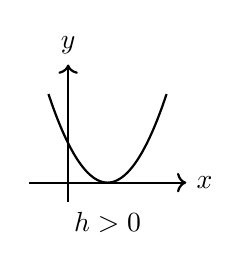
\begin{tikzpicture}[
            scale=0.5,
            declare function={
                func(\x) = (\x-1)*(\x-1);
            }
        ]
            \draw[->, thick] (-1, 0) -- (3, 0) node[right] {$x$};
            \draw[->, thick] (0, -0.5) node[below, xshift=0.5cm] {$h>0$} -- (0, 3) node[above] {$y$};
        
            \draw[domain=-0.5:2.5, smooth, thick, variable=\x] plot ({\x}, {func(\x)});
            
        \end{tikzpicture}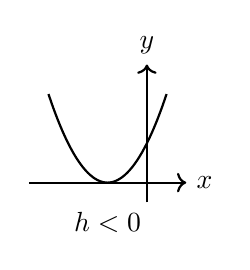
\begin{tikzpicture}[
            scale=0.5,
            declare function={
                func(\x) = (\x+1)*(\x+1);
            }
        ]
            \draw[->, thick] (-3, 0) -- (1, 0) node[right] {$x$};
            \draw[->, thick] (0, -0.5) node[below, xshift=-0.5cm] {$h<0$} -- (0, 3) node[above] {$y$};
        
            \draw[domain=-2.5:0.5, smooth, thick, variable=\x] plot ({\x}, {func(\x)});
            
        \end{tikzpicture}
};
\node (k) [right of=start,yshift=-1.5cm] {
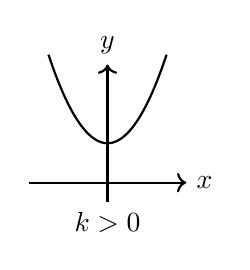
\begin{tikzpicture}[
            scale=0.5,
            declare function={
                func(\x) = \x*\x+1;
            }
        ]
            \draw[->, thick] (-2, 0) -- (2, 0) node[right] {$x$};
            \draw[->, thick] (0, -0.5) node[below] {$k>0$} -- (0, 3) node[above] {$y$};
        
            \draw[domain=-1.5:1.5, smooth, thick, variable=\x] plot ({\x}, {func(\x)});
            
        \end{tikzpicture}
        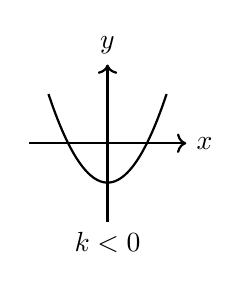
\begin{tikzpicture}[
            scale=0.5,
            declare function={
                func(\x) = \x*\x-1;
            }
        ]
            \draw[->, thick] (-2, 0) -- (2, 0) node[right] {$x$};
            \draw[->, thick] (0, -2) node[below] {$k<0$} -- (0, 2) node[above] {$y$};
        
            \draw[domain=-1.5:1.5, smooth, thick, variable=\x] plot ({\x}, {func(\x)});
            
        \end{tikzpicture}
};

\draw [arrow] (start) -- node[anchor=south, yshift=0.5cm] {$y=(x-h)^2$} (h);
\draw [arrow] (start) -- node[anchor=north, yshift=-0.5cm] {$y=x^2+k$} (k);
\end{tikzpicture}
\end{center}

看图像可以得出当\(a>0\)时,抛物线顶点的纵坐标是函数的最小值;当\(a<0\)时,抛物线顶点的纵坐标是函数的最大值

如果已知抛物线的顶点坐标和抛物线上的另外一个点就能求出抛物线的解析式


\begin{example}
    已知二次函数 \(y = ax^2 + bx + c\),当 \(x = -3\) 时,函数值取得最值 \(4\),当 \(x = 1\) 时,\(y = -8\),则这个二次函数的解析式为\underline{\hspace{5em}}.
    \begin{solution}
        分析:由\(x=-2\),函数值取得最值\(4\)知道抛物线的顶点坐标为\((-3, 4)\),还提供了抛物线上的另外一个点\((1, -8)\),所以确定用顶点式求解析式更快,所以先设解析式\(y=a(x-h)^2+k\),再代入\(h,k\)的值,然后只剩参数\(a\),代入另外一个点\((1, -8)\)即可求得解析式.设解析式为$y = a(x - h)^2 + k$再代入 \(h, k\) 的值,只剩参数 \(a\),代入另一点即可求出.

        
        \[
\begin{alignedat}{3}
&\text{设解析式为 } y = a(x - h)^2 + k, &\quad
&\because x = -3 \text{ 时函数值取得最值 } 4, &\quad
&\therefore \text{顶点为 } (-3,4), \\[2pt]
&\therefore y = a(x+3)^2 + 4, &
&\because (1,-8) \text{ 在抛物线上}, &
&-8 = a(1+3)^2 + 4, \\[2pt]
&-8 = 16a + 4, &
&16a = -12, &
&a = -\dfrac{3}{4}, \\[2pt]
&\therefore y = -\frac{3}{4}(x+3)^2 + 4, &
&= -\frac{3}{4}(x^2 + 6x + 9) + 4, &
&= -\frac{3}{4}x^2 - \frac{9}{2}x - \frac{27}{4} + \frac{16}{4}, \\[2pt]
& & & & &y = -\frac{3}{4}x^2 - \frac{9}{2}x - \frac{11}{4}
\end{alignedat}
\]

        
        
    \end{solution}
\end{example}


%顶点式的关键是顶点坐标为(h,k)

\subsection{一般式}
二次函数一般式:\(y=ax^2+bx+c\).

顶点式实际上由一般形式配方而来, 二次函数的顶点式常用于直观表现出二次函数的顶点, 一般式主要体现抛物线与系数的关系:


二次函数的一般式为:
\[
y = ax^2 + bx + c\quad (a \neq 0)
\]
其中,$a$、$b$、$c$ 为常数,$a$ 决定开口方向与宽窄,$b$ 影响对称轴位置,$c$ 为纵截距(截距指函数与y轴的交点的纵坐标).

二次函数的一般式可以通过配方化为顶点式 $y = a(x - h)^2 + k$,其中 $(h,k)$ 为顶点坐标.

从一般式出发:
\[
y = ax^2 + bx + c
\]
提取 $a$:
\[
y = a\left(x^2 + \frac{b}{a}x\right) + c
\]
在括号内配方:
\[
y = a\left[x^2 + \frac{b}{a}x + \left(\frac{b}{2a}\right)^2 - \left(\frac{b}{2a}\right)^2 \right] + c
\]
整理:
\[
y = a\left(x + \frac{b}{2a}\right)^2 - \frac{b^2}{4a} + c
\]
由此得到顶点式:
\[
y = a\left(x + \frac{b}{2a}\right)^2 + \left(c - \frac{b^2}{4a}\right)  \quad\Rightarrow\quad y = a\left(x + \frac{b}{2a}\right)^2 + \frac{4ac-b^2}{4a}
\]
可以推出顶点坐标为:
\[
h = -\frac{b}{2a}, \quad k = \dfrac{4ac-b^2}{4a}
\]

如果已知一般式要求顶点不想配方,就可以套用$h = -\dfrac{b}{2a}, \quad k = \dfrac{4ac-b^2}{4a}$,一般式也可以反映对称轴即顶点的横座标:\(x=-\dfrac{b}{2a}\)
总结一般式的性质如下:
\begin{enumerate}
    \item 对称轴:$x = -\dfrac{b}{2a}$
    \item 顶点:$\left(-\dfrac{b}{2a},\ \dfrac{4ac-b^2}{4a}\right)$
    \item 开口方向:$a > 0$ 向上开口;$a < 0$ 向下开口
\end{enumerate}

%%%%%%%%%%%%%%%%%%%%%%%%%%%%%%%%%%%%%%%%%%%%%%%%%%%%%%%%%%%%%%%%%%%%%%%%%%%%%%%%%此处未遍例题

“一般式主要体现抛物线与系数的关系”,你是否联想到了韦达定理(根与系数的关系)?


\subsection{交点式(两根式/因式分解式)}
\textbf{交点式:\(y=a(x-x_1)(x-x_2) \quad (\Delta>0)\)}

交点式常用于直观表现直观表现二次函数与\(x\)轴的交点坐标.

\textbf{推导:}二次函数的一般式为:
\[
y = ax^2 + bx + c, \quad a \neq 0
\]
如果它在 $x$ 轴上有两个实数交点 $x_1$ 和 $x_2$(即二次方程 $ax^2 + bx + c = 0$ 有实根),
那么函数可以写成交点式(因式分解式):
\[
y = a(x - x_1)(x - x_2)
\]


设二次方程 $ax^2 + bx + c = 0$ 的两个实根为 $x_1$ 和 $x_2$,由韦达定理:
\[
x_1 + x_2 = -\frac{b}{a}, \quad x_1 x_2 = \frac{c}{a}
\]
则:
\[
ax^2 + bx + c 
= ax^2-\dfrac{b}{a}x+\dfrac{c}{a}
= \underbrace{a\left[x^2 - (x_1 + x_2)x + x_1 x_2\right]}_{\text{提取公因数\(a\)}}
\]
代入根与系数关系:
\[
= a\left[x^2 - \left(-\frac{b}{a}\right)x + \frac{c}{a}\right]
= a\left(x - x_1\right)\left(x - x_2\right)
\]
所以二次函数的交点式为:
\[
y = a(x - x_1)(x - x_2)
\]

交点式便于直接观察函数与\(x\)轴的交点,由于教材没有介绍交点式,所以不要在书写题目过程的时候使用交点式,可以在选填或检验的时候使用交点式快速得到答案.

使用交点式的前提是$\Delta > 0$,特别的,\textbf{当\(\Delta=0\)时,交点式退化为$y = a(x - p)^2$},如果$\Delta < 0$,由于二次函数与\(x\)轴无交点,所以不能写成交点式,需要根据情况写成顶点式或一般式.总结交点式的性质如下:

\begin{enumerate}
    \item 交点式中的 $x_1$、$x_2$ 为函数图像与 $x$ 轴的交点横坐标.
    \item 当 $a > 0$ 时,抛物线开口向上;当 $a < 0$ 时,抛物线开口向下.(与顶点式和交点式相同)
    \item 交点式可直观反映零点位置与图像对称性.(零点指二次函数\(y=ax^2+bx+c\)的\(y=0\)时\(x\)的值,即方程\(ax^2+bx+c=0\)的解)
\end{enumerate}

%%%%%%%%%%%%%%%%%%%%%%%%%%%%%%%%%%%%%%%%%%%%%%%%%%%%%%%%未编写例题
%二次函数区间最值
\section{二次函数区间最值}

区间可以简单理解为一段连续的取值范围.

%二次函数交点
\section{二次函数与坐标轴、直线的交点}

本节探讨二次函数与坐标轴或任意直线的交点有关的问题.分为两类,一类是与线段、射线或直线的交点,另一类是与坐标轴的交点
\subsection{与线段、射线或直线的交点}
这类题目通常会提供一个含参的二次函数和一个范围(区间、直线、坐标轴或其他),然后探讨参数取何值能使二次函数与这个范围有一个交点、两个交点或没有交点.
\subsubsection*{代数思想}

%%%%%%%%%%%%%%%%%%%%%%%%%%%%%%%%%%%%%%%%%%%%函数中的定值
%横轴上一点,二次项系数开口向下,一定有两个交点

%定点在横轴上,必定只有一个交点

%函数里的k必须能被“抵消”掉(即含k的式子能等于 0)时,函数过定点

%---------------------------------------开始分类


首先要观察表达式中提供的信息,例如二次函数过某一定点、开口方向、对称轴等等信息,利用已知信息会减少下来不必要的分类讨论.把二次函数限定在横轴上要从四个方面考虑:
\begin{itemize}
    \item \textbf{开口方向}(这是分类的前提条件)
    \item \textbf{判别式}(限定根的情况)
    \item \textbf{对称轴}(根的值不确定时,限定范围)
    \item \textbf{范围端点}(紧接对称轴限定的范围继续限定在范围的两个端点内)
\end{itemize}

一般来说并不是四个都需要考虑,需要结合已知条件讨论.

\exas{
已知抛物线 \( y = x^2 - kx - k \),\( A (1, -2) \),\( B (4, 10) \).抛物线与线段 \( AB \)(包括 \( A \),\( B \) 两点)有两个交点,则 \( k \) 的取值范围为\underline{\hspace{4.5em}}.
}{




}

\begin{example}
已知抛物线 \( y_1 = mx^2 + 4x - 2 \) (\( m \neq 0 \)) 的顶点为 \( C \).已知点 \( M(-1, -4), N(3, 0) \),若该抛物线与线段 \( MN \) 总有两个不同的交点,请求出 \( m \) 的取值范围.
\end{example}

%1确定开口方向
%+
%有无定量(过定点)
%可以得出
%横轴上下一点,二次项系数开口向下或向下,一定有两个交点


%------------------------------------------卡交点

在确定开口方向的情况下234

2确定判别式的情况(限定在横轴上有无交点/有几个交点)
二次函数与横轴的交点的横坐标实际上是\(y=0\)时\(x\)的值,可以看作是一个一元二次方程,要判断这个二次函数与横轴有没有交点.实际上就是判断一元二次方程有没有实数根,使用根的判别式\(\Delta\)就能解决.结合"求根公式法"这一章就知道如果有一个交点那么\(\Delta=0\),如果有两个交点,则\(\Delta>0\)

%-------------------------------------------卡范围


3确定对称轴在题目给定的范围内


4范围两端点




恒等变形转化为与横轴的交点






\subsubsection*{图像思想}

前面我们使用代数思想分析交点类的问题,使用代数法解决交点问题比较通用.但在遇到已知条件较为充足时可以采用数形结合的思想快速解决此类问题,适用于条件丰富无需分类讨论的题目,缺点是不能适用于所有题目,比较局限.

\begin{example}
一段抛物线 \( L: y = -x (x-3) + c \)\( (0 \leq x \leq 3) \) 与直线 \( l: y = x + 2 \) 有唯一公共点,则 \( c \) 的取值范围为\underline{\hspace{4em}}。
\end{example}

\subsection{与坐标轴的交点}
明确交点类型
分类讨论函数类型
分析交点总数
特殊情形处理

检查函数是否通过原点(0,0)

检查与y轴交点是否同时也是与x轴交点


%二次函数实际问题
\section{二次函数实际问题}


\subsection{有关图形}

有关图形的问题比较多样.重点在于理解问题,一般来说需要一步一步地将几个量的表达式推导出来(利用数量关系、利用几何关系).有些题目的数量关系比较复杂,捋清楚关系才能得到表达式,同时不能忽略自变量的取值范围.

本节给不同的题目进行分类,看似复杂实际上都是一样的底层逻辑.


\subsubsection*{围墙}


\begin{wrapfigure}{r}{3cm}
    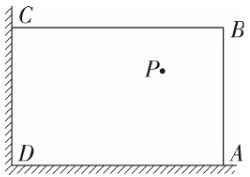
\includegraphics[width=1\linewidth]{figure/p1.png}
    \caption{}
    \label{fig:p1}
\end{wrapfigure}

\exas{
如图\ref{fig:p1},某劳动小组借助一个直角墙角围成一个矩形劳动基地 $ABCD$,墙角两边 $DC$ 和 $DA$ 足够长,用总长 $28\ \text{m}$ 的篱笆围成另外两边 $AB$ 和 $BC$,有下列结论:

\begin{enumerate}
    \item 当 $AB$ 的长是 $10\ \text{m}$ 时,劳动基地 $ABCD$ 的面积是 $180\ \text{m}^2$;
    \item $AB$ 的长有两个不同的值满足劳动基地 $ABCD$ 的面积为 $192\ \text{m}^2$;
    \item 点 $P$ 处有一棵树(树的粗细忽略不计),它到墙 $DC$ 的距离是 $12\ \text{m}$,到墙 $DA$ 的距离是 $8\ \text{m}$,如果这棵树需在劳动基地内部(包括边界),那么劳动基地面积的最大值是 $196\ \text{m}^2$,最小值是 $160\ \text{m}^2$.
\end{enumerate}

其中,正确结论的个数是(\hspace{3.5em})

\begin{enumerate*}[label=\Alph*.]
    \item 0 \hspace{3em}
    \item 1 \hspace{3em}
    \item 2 \hspace{3em}
    \item 3
\end{enumerate*}
}{
分析:(1)先要知道边\(AB\)与面积的关系,所以设\(AB\)为自变量\(x\),因为总长为28,所以\(BC\)的长为\((28-x)\),所以\(y=x(28-x)\),将\(10\)代入,求得结果确实是180所以正确.(2)前面得出了\(y=x(28-x)\),这里问边长\(AB\)与面积的关系所以继续使用\(y=x(28-x)\)表达,接着代入\(192\)到函数,思路一:计算判别式,看\(x(28-x)=0\)与\(y=192\)是否有两个交点,思路二:因式分解解方程,如果结果有两个,则确实有两个不同的值满足条件.经过计算(2)正确.(3)由题意可知\(\begin{cases}
x>8\\
28-x>12
\end{cases}\)解得\(8\le x \le 16\)是关于\(x\)的区间,将\(x=8\)和\(x=16\)分别代入函数\(y=x(28-x)\),分别得到160和192,所以函数的最小值应该是160,因为函数开口向下,所以顶点纵座标是函数最大值,将函数化为顶点式得\(y=-(x-14)^2+196\),所以最大值为196.以上三个选项都正确,故选\(D\)
}


\begin{wrapfigure}{r}{3cm}
    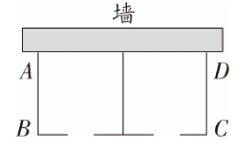
\includegraphics[width=1\linewidth]{figure/p2.png}
    \caption{}
    \label{fig:p2}
\end{wrapfigure}

\subsubsection*{分割}

\exas{
如图\ref{fig:p2},园林部门计划在某公园建一个长方形苗圃 $ABCD$,苗圃的一面靠墙(墙最大可用长度为 $14\ \text{m}$),另三边用木栏围成,中间也用垂直于墙的木栏隔开,分成两个区域,并各留 $2\ \text{m}$ 宽的门(门不用木栏),若建成后所用木栏总长为 $32\ \text{m}$,则长方形 $ABCD$ 的最大面积为(\hspace{3.5em})
\begin{enumerate*}[label=\Alph*.]
    \item $\dfrac{22}{3}\ \text{m}^2$ \hspace{3em}
    \item $108\ \text{m}^2$ \hspace{3em}
    \item $\dfrac{318}{3}\ \text{m}^2$ \hspace{3em}
    \item $\dfrac{308}{3}\ \text{m}^2$
\end{enumerate*}
}{
分析:要求面积最值,实际上是要先求边与面积的关系,题目没有给出具体边长,所以这里需要设完整的两条边来求,可以选择先设\(AB,DC\)或\(AD\),这里示例设\(AB\)为\(x\),要求面积还需要另外一条完整的边,因为留了2m的门(注意这里有两个门是4m)、墙的一面没有用木栏围住、中间用长\(x\)的木栏隔开(平行线间的距离处处相等),设中间的隔板为\(MN\),所以加上\(32+2\times2=36\)的长是\(AB+BC+CD+MN=36\),代入\(x\)得\(3x+BC=36\),所以\(BC=AD=36-3x\),这里题目还要求墙的最长为\(14\)所以\(36-3x\le14\)解得\(x\ge\dfrac{22}{3}\).表示出长和宽就能表示\(ABCD\)的面积为\(y=x(34-x)\ (x\ge\dfrac{20}{3})\),此时就将面积最值问题转化为区间最值问题(注意这里的区间范围不能使用顶点式求最值).解得最大值为\(\dfrac{308}{3}\), 故\(D\)正确.
}

\begin{wrapfigure}{r}{3cm}

    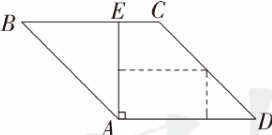
\includegraphics[width=1\linewidth]{figure/p3.png}
    \caption{}
    \label{fig:p3}
    
\end{wrapfigure}

\exas{
如图\ref{fig:p3},是一块菱形新型平面材料 \(ABCD\),
\(\angle BAD = 135^\circ\),\(AB = 50\ \text{cm}\),点 \(E\) 在 \(BC\) 上,且
\(EA \perp AD\),先沿着 \(AE\) 切开材料,然后在四边形 \(ADCE\) 内切割出一块矩形,且矩形相邻两条边分别落在 \(AD\)、\(AE\) 上,一个顶点落在 \(CD\) 边上.设边 \(AE\) 上矩形的边长为 \(x\ \text{cm}\),矩形的面积为 \(y\ \text{cm}^2\),有下列结论:

\begin{enumerate}
    \item \(y\) 与 \(x\) 之间的函数解析式为 \(y = -x^2 + 50x \quad (0 < x \leq 25\sqrt{2})\);
    \item 当 \(x = 10\) 时,切割出矩形后,四边形 \(AECD\) 剩余的面积为 \((1250\sqrt{2} - 625)\ \text{cm}^2\);
    \item 若切割出的矩形材料用于某种生产时,售价为 \(1.5\ \text{元}/\text{cm}^2\),则当 \(x = 25\) 时,出售此块矩形材料的总价最大,最大值为 \(937.5\ \text{元}\).
\end{enumerate}

其中,正确结论的个数是\(\underline{\hspace{3em}}\).

\begin{enumerate*}[label=\Alph*.]
    \item 0 \hspace{3em}
    \item 1 \hspace{3em}
    \item 2 \hspace{3em}
    \item 3
\end{enumerate*}

}{
\begin{wrapfigure}{r}{3cm}
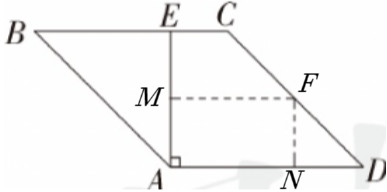
\includegraphics[width=1\linewidth]{figure/p3-1.png}
    \label{fig:p3_1}
    \caption{}
\end{wrapfigure}
分析:在正式分析之前需要先将题目所给得信息正利好,已知菱形中一个角\(\angle BAD=135^\circ\),推导能得出\(\angle B= \angle D=45^\circ\),因为\(AB=50cm\)所以其他三条边也是\(50cm\).(1)要验证解析式是否正确,实际上是要用边长与面积的关系构造函数,如图设点\(M,F,N\),则\(AM=x\),还要注意\(x\)所在的范围,因为四边形\(ABCD\)是矩形,所以\(A,B,C,D\)四点不共线,也就是说\(M\)不与\(A\)重合,\(F,N,D\)都不重合,所以\(x>0\),因为切割的矩形在菱形内,所以\(MA\le EA\),根据已知信息可以推导\(EA=25\sqrt{2}\),综合起来\(0<x\le25\sqrt{2}\).表示出\(MA\)后就要表示矩形的另外一边,这里选择表示\(AN\)比较方便,因为推导可得\(ND=FN=x\),又\(AD=50cm\),所以\(AN=AD-ND=50-x(cm)\),所以切割矩形面积的函数\(y=x(50-x)\quad(0<x\le25\sqrt{2})\),整理为一般形式\(y=-x^2+50x\quad(0<x\le25\sqrt{2})\),故(1)正确.

(2)要求证剩余面积,实际上是问切割矩形的面积与剩余面积的关系:剩余面积=四边形\(AECD\)面积-切割矩形面积.以此构造函数,最后代入\(x=10\) ,得到结果\(1250\sqrt{2}-1025\).故(2)错误.

(3)要求售价最大,实际上是问单价与切割面积的关系,以此构造函数\(w=1.5(-x^2+50x)\quad (0<x\le25\sqrt{2})\),将其整理为一般形式\(w=-\dfrac{3}{2}x^2+75\quad (0<x\le25\sqrt{2})\) 因为该函数开口向下所以有最大值,将其整理为顶点式得到\(w=-1.5(x-25)+937.5\) ,因此当\(x=25\)时确实取最大值,且最大值确实为\(937.5\) ,故(3)正确

综上,有两个结论正确,故选\(C\)
}

\subsubsection*{动点}

\begin{wrapfigure}{r}{3cm}
\vspace{-1cm}
    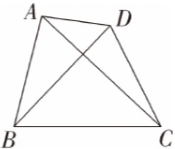
\includegraphics[width=1\linewidth]{figure/p4.png}
    \caption{}
    \label{fig:p4}
\end{wrapfigure}

\exas{
如图\ref{fig:p4},某公园的示意图是对角线互相垂直的四边形 \(ABCD\),已知 \(AC+BD=160\) 米,则该四边形公园的最大面积为\underline{\hspace{3.5em}}平方米.

}{
要求面积最大值,首先要列出面积的表达式,观察图形,可以将该四边形分为两个三角形,这里以\(\triangle ABC\)与\(\triangle ADC\)为例,设\(AC\)与\(BD\)相交于点\(M\),就能顺利构造函数\(s=S_{\triangle ABC}+S_{\triangle ADC}=\dfrac{1}{2}AC \cdot BM + \dfrac{1}{2}AC \cdot DM\),整理得\(s=\dfrac{1}{2}AC \cdot BD\).接下来就需要表示\(AC\)和\(BD\) .根据\(AC+BD=160\),设\(AC\)为\(x\)则\(BD\)为\(160-x\),所以\(s=\dfrac{1}{2}x(160-x)\)整理得\(s=-\dfrac{1}{2}x^2+80x\).因为该函数开口向下,所以有最大值,将其写为顶点式,计算得最最大值为\(3200m^2\) ,故四边形公园的最大面积为\(3200m^2\)



}

\begin{wrapfigure}{r}{3cm}
\vspace{-1.8cm}
    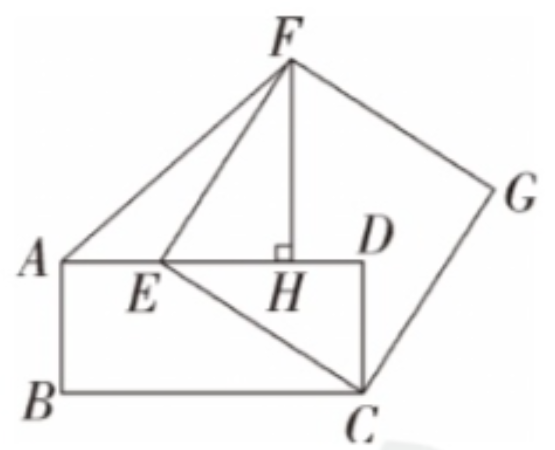
\includegraphics[width=1\linewidth]{figure/p5.png}
    \caption{}
    \label{fig:p5}
\end{wrapfigure}


\begin{example}
    如图\ref{fig:p5},在矩形 \(ABCD\) 中,\(AD=4\),\(E\) 是 \(AD\) 边上的动点,连接 \(CE\),以 \(CE\) 为边向右上方作正方形 \(CEFG\),过点 \(F\) 作 \(FH \perp AD\),垂足为点 \(H\),连接 \(AF\).在整个变化过程中,\(\triangle AEF\) 面积的最大值是\underline{\hspace{3.5em}}.
\end{example}

\begin{wrapfigure}{r}{3cm}
    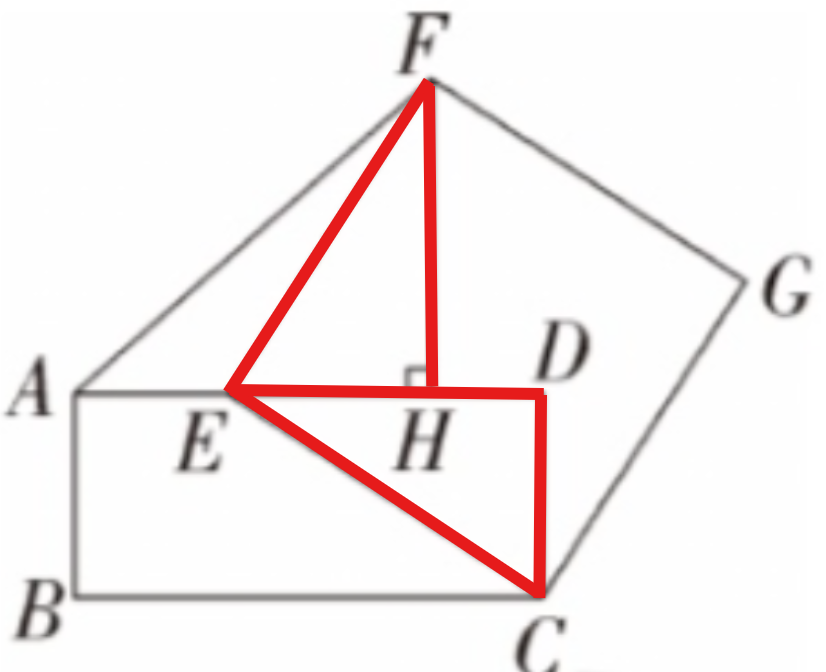
\includegraphics[width=1\linewidth]{figure/p5-1.png}
    \caption{}
    \label{fig:p5_1}
\end{wrapfigure}

\begin{solution}
分析:首先构造\(\triangle AEF\)面积的函数\(s=\dfrac{1}{2}AE\cdot FH\),接下来就要建立\(AE\)和\(FH\)的联系.观察图形,可知\(AE=AD-ED=4-ED\),就将\(AE\)转化为先求\(ED\),观察图形(如图\ref{fig:p5_1})可以发现\(ED\)与\(FH\)存在联系,通过“一线三垂直”推导可得\(ED=FH\),所以设\(FH=x\),则\(AE=4-x\),注意\(x\)的取值,因为\(E\)是\(AD\)上的动点,所以\(0\le4-x\le4\),化简得\(0\le x\le 4\),代入函数解析式得\(s=\dfrac{1}{2}x(4-x)\quad(0\le x\le 4)\),将其写为顶点式,当\(x=2\)时,函数\(s\)取得最大值是2,且在区间内是最大值符合题意.故\(\triangle AEF\) 面积的最大值是2

\end{solution}


\subsection{有关商品销售}



\exas{
某商场要经营一种新上市的文具,进价为10元/件.试营销阶段发现:当销售单价为20元时,每天的销售量是200件;销售单价为30元时,每天的销售量是100件.其中每天的销售量是售价的一次函数.

\begin{enumerate}[label=(\arabic*)]
    \item 求这种文具每天的销售量 $y$ (件) 与销售单价 $x$ (元) 之间的函数解析式;
    
    \item 销售单价为多少元时,该文具每天的销售利润最大?
\end{enumerate}
}{
分析:(1)已知单售价为自变量,销售量为因变量,由题意知他们的关系式是一次函数,所以设\(y=kx+b\),代入题目所给数据求出解析式为\(y=-10x+400\)
(2)首先明确要求销售利润与单价的关系式,要知道每日销售利润=单品利润\(\times\)每日总销售量,单品利润=单品售价-单品进价,那么由题意得单品利润为\(x-10\) ,每日销售量为\(-10x+400\),即可构造函数\(w=(x-10)(-10x+400)\) ,整理得\(w=-10x^2+500x-4000\),将其写为顶点式,得当\(x=25\)时,函数取得最大值2250 .

}


\begin{wrapfigure}{r}{6cm}
    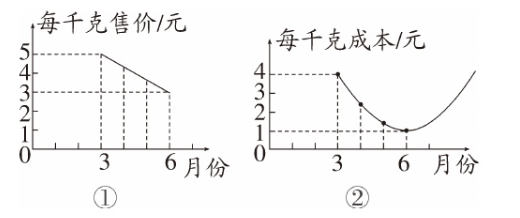
\includegraphics[width=1\linewidth]{figure/p7.png}
    \caption{}
    \label{fig:p7}
\end{wrapfigure}

\exas{
某种蔬菜的销售单价与销售月份之间的关系如图\textcircled{1}所示,成本与销售月份之间的关系如图\textcircled{2}所示(图\textcircled{1}的图象是线段,图\textcircled{2}的图象是抛物线).\underline{\hspace{1cm}}月出售这种蔬菜,每千克的收益最大.(收益=售价-成本)
}{
分析:题目给出售价与月份的关系和成本与月份的关系,如果知道售价的解析式和成本的解析式,代入收益=售价-成本就能表示出收益的解析式,写成顶点式的形式就能取得最值.由题意和图像可以知道售价和成本都受月份影响,所以将月份作为自变量\(x\),售价和成本分别为两个函数\(y_1,y_2\),图中给出\(y_1,y_2\)上一些点的坐标,分别求出\(y_1,y_2\)的解析式,设收益为\(w\)则\(w=y_1-y_2\),再对\(w\)配方取得最值.最后注意题目问的是月份,不要写成最值.
}





\subsection{有关抛物线形状}


\begin{wrapfigure}{r}{6cm}
    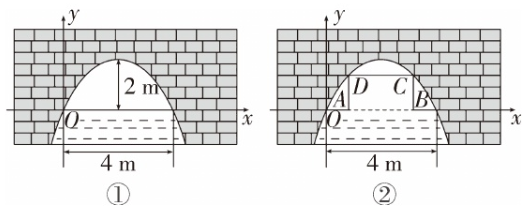
\includegraphics[width=1\linewidth]{figure/p8.png}
    \caption{}
    \label{fig:p8}
\end{wrapfigure}

\exas{
如图\ref{fig:p8}为抛物线形拱桥平面示意图,拱顶离水面 2 m,水面宽 4 m.以现有水平面的水平直线为 \( x \) 轴,与抛物线形拱桥左边交点为原点建立平面直角坐标系.

\begin{enumerate}
    \item 求此抛物线解析式.
    
    \item 如图\textcircled{1},若水面下降1 m,水面宽度增加多少米?
    
    \item 如图\textcircled{2},为保证行船安全,在汛期来临之前,管理部门需要用一定长度的钢板搭建一个可调节大小的矩形"安全架",露出水平面部分为 \( AD-DC-CB \),使点 \( C, D \) 在抛物线上,点 \( A, B \) 为露出水面的端点,若确保点 \( A, B \) 的间距不少于3 m,求 \( AD-DC-CB \) 的最大长度.
\end{enumerate}
}{}

\begin{wrapfigure}{r}{6cm}
    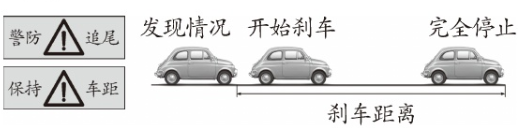
\includegraphics[width=1\linewidth]{figure/p9.png}
    \caption{}
    \label{fig:p9}
\end{wrapfigure}

\exas{
随着时代的进步,我国交通出行结构发生根本性变化,汽车出行成为交通常态.某数学兴趣小组观察校门口的汽车发现,很多车尾部贴上了保持车距的贴纸.小组成员产生了一个困惑——"保持怎样的车距才能保障道路安全?"为解决这一困惑,小组成员分工开展活动:
成员小梧查阅某型号汽车官网数据得到汽车行驶速度 $x$ (m/s) 与刹车距离 $y$ (m) 的关系如表(刹车距离:从发现前方道路有异常情况到车辆完全停止所行驶的距离.)

\begin{table}[h]
\centering
\caption{某型号汽车行驶速度 $x$(m/s) 与刹车距离 $y$(m) 的关系}
\begin{tabular}{|c|c|c|c|c|c|c|c|}
\hline
行驶速度 $x$/(m/s) & 0 & 5 & 10 & 15 & 20 & 25 & 30 \\
\hline
刹车距离 $y$/m & 0 & 3.25 & 9 & 17.25 & 28 & 41.25 & 57 \\
\hline
\end{tabular}
\end{table}

\begin{itemize}
    \item 任务1:小梧认为该型号汽车的行驶速度 $x$ (m/s) 与刹车距离 $y$ (m) 之间存在函数关系,请你协助小梧求出该函数解析式.
    \item 任务2:成员小杭发现小区门口路段限速60 km/h.请你帮小杭计算,如果该型号汽车以最高限速60 km/h行驶,至少保持多少车距才能保障道路安全?
    \item 任务3:实际驾驶过程中,驾驶员难以预估前车的距离,且难以实时计算不同行驶速度对应的安全距离,是否存在简单、实用且能维持适当安全距离的方案?小组成员带着困惑与陈老师进行交流,陈老师分享了他保持车距常用的方案"2秒定律"——跟车行驶时设定一个参照物,前车超越参照物后,后车如果在两秒内到达该参照物,说明与前车的距离不足,反之距离充足.
\end{itemize}
}{}

%%%%%%二次函数与几何
\section{二次函数与几何}



\subsection{二次函数的几何变换}

\subsubsection*{平移}
还记得平移运动吗?简单回顾:平移是全等的几何变换(平移前和平移后的图形全等),平移具有交换性(比如一个正方形先向上平移3个单位再向左平移3个单位,如果颠倒顺序,最终位置相同)和可逆性(平移后可以通过反向平移回到原位置).
\par
对二次函数平移其实就是\textbf{对二次函数的顶点平移}(请回顾小节\ref{subsetionL:topponit}-顶点式),进行任何平移操作前需要先把二次函数化为顶点式以方便操作.
\par
假设有\(y=a(x-h)^2\),若\(h>0\)则函数向左平移,若\(h<0\)则函数向右平移,都是平移\(|h|\)个单位;假设有\(y=ax^2+k\),若\(k>0\)则函数向上平移,若\(k<0\)则函数向下平移,都是平移\(|k|\)个单位.两者一起进行就是顶点式\(y=a(x-h)^2+k\).
\par
\begin{example}抛物线\( l_1 \)是由抛物线\( l_2 \)向下平移3个单位长度,再向左平移2个单位长度得到的,已知抛物线\( l_1 \)的解析式为\( y=2(x-2)^2+3 \),则抛物线\( l_2 \)的解析式为(\hspace{3.5em})

\begin{enumerate}[label=\Alph*.]
    \item \( y=2(x-4)^2+6 \)
    \item \( y=2(x-2)^2 \)
    \item \( y=2x^2+6 \)
    \item \( y=2x^2 \)
\end{enumerate}
\end{example}
\begin{solution}
    分析:因为1由2向下平移3个单位再向左平移2个单位,题目已知1求2,只需对1进行反向操作,即向右平移2个单位再向上平移3单位,经过计算A正确.
\end{solution}
以上是抛物线沿坐标轴方向平移的例子,如果沿斜向(即直线)平移呢?这时候只要知道平移的距离和直线的解析式,过移动后的顶点做垂线,垂直于坐标轴,就能\textbf{构造一个直角三角形}.根据直线解析式,\textbf{设移动后顶点的坐标},顶点的横纵坐标值就是三角形直角边的长,最后通过\textbf{勾股定理}就能得出移动后顶点的坐标.
\begin{example}
    将抛物线 \( y = x^2 \) 沿直线 \( y = 3x \) 方向移动 \(\sqrt{10}\) 个单位长度,若移动后抛物线的顶点在第一象限,则移动后抛物线的解析式是\underline{\hspace{4em}}.
\end{example}
\begin{solution}
    分析:该二次函数沿一条直线移动,没有指定移动的方向,但题目要求移动后二次函数的顶点在第一象限,因为该直线(正比例函数)的斜率为\(3>0\),\(x>0\)时\(y\)随\(x\)的增大而增大,所以只有在二次函数往右上方移动时才符合题意(可以画草图辅助理解,如图\ref{fig:move1}),此时根据正比例函数可以设移动后的坐标为\((m,3m)\),再作\(BA\)垂直于\(x\)轴,原点为点\(C\),移动后的定点坐标为\(B\),\(BA=3m,CA=m,CB=\sqrt{10}\),利用勾股定理即可求出移动后的顶点坐标,根据顶点坐标列成顶点式再化为一般式即可.
    \par
    \begin{figure}[h]
        \centering
    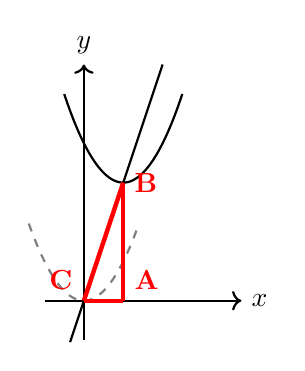
\begin{tikzpicture}[scale=0.5]
    % 绘制坐标系
                                        \draw[->, thick] (-1,0) -- (4,0) node[right] {$x$}; % x轴
                                        \draw[->, thick] (0,-1) -- (0,6) node[above] {$y$}; % y轴
                                        \draw[domain=-1.4:1.4, smooth, dashed, thick, gray] plot (\x, {\x*\x}); % 标注函数
                                        \draw[domain=-0.35:2, smooth, thick] plot (\x, {\x*3}); % 标注函数
                                        \draw[domain=-0.5:2.5, smooth, thick, black] plot (\x, {(\x - 1)^2 + 3}); % 标注函数
                                        \draw[red, ultra thick] (0,0) node[above left] {$\textbf{C}$} -- (1,3) node[right] {$\textbf{B}$};
                                        \draw[red, ultra thick] (1,0) node[above right] {$\textbf{A}$} -- (1,3);
                                        \draw[red, ultra thick] (0,0) -- (1,0);
    \end{tikzpicture}
    \caption{}
        \label{fig:move1}
    \end{figure}
\end{solution}


\noindent
\begin{minipage}{1\linewidth}
\begin{wrapfigure}{r}{3cm}
    \vspace{-2cm}
    \centering
    \begin{minipage}{1\linewidth}
    \centering
        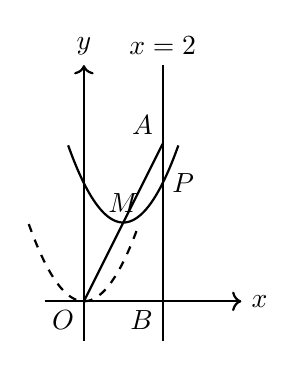
\begin{tikzpicture}[scale=0.5] % 整体缩放
                                        % 绘制坐标系
                                        \draw[->, thick] (-1,0) -- (4,0) node[right] {$x$}; % x轴
                                        \draw[->, thick] (0,-1) -- (0,6) node[above] {$y$}; % y轴
                                        % 标注原点 O
                                        \node at (0,0) [below left] {$O$};
                                        % 绘制点 A(2,4)
                                        \filldraw (2,4) circle (0pt) node[above left] {$A$};
                                        % 绘制直线 x=2(虚线)
                                        \draw[thick] (2,-1) -- (2,6) node[above] {$x=2$};
                                        % 绘制点 B(2,0)
                                        \filldraw (2,0) circle (0pt) node[below left] {$B$};
                                        % 绘制直线 OA(实线)
                                        \draw[thick] (0,0) -- (2,4) node[midway, above left, black] {}; % 不额外标注
                                        % 绘制初始二次函数 y=x^2(虚线,示意原始位置)
                                        \draw[domain=-1.4:1.4, smooth, dashed, thick] plot (\x, {\x*\x}); % 标注函数
                                        % 绘制平移后的二次函数(示例:顶点 M 在 (1,2) 处)
                                        % 函数解析式:y = (x-1)^2 + 2 = x^2 - 2x + 3
                                        \draw[domain=-0.4:2.4, smooth, thick] plot (\x, {(\x-1)^2 + 2}); % 标注
                                        % 标注顶点 M(1,2)
                                        \filldraw (1,2) circle (0pt) node[above] {$M$};
                                        % 标注点 P(2,3)(二次函数与 x=2 的交点)
                                        \filldraw (2,3) circle (0pt) node[right] {$P$};
                                        
                                        \end{tikzpicture}
                                        \par
    题图1
    \end{minipage}
    \end{wrapfigure}
\begin{minipage}{1\linewidth}
\begin{exercise}
    \small
    \setlength{\parindent}{0pt} % 取消段落缩进
    \setlength{\columnseprule}{0.01pt}
    \begin{multicols}{2}
    (1)如题图1,在平面直角坐标系中,已知点 \( A \) 坐标为 \((2,4)\),直线 \( x=2 \) 与 \( x \) 轴相交于点 \( B \),连接 \( OA \),二次函数 \( y=x^2 \) 图象从点 \( O \) 沿 \( OA \) 方向平移,与直线 \( x=2 \) 交于点 \( P \),顶点 \( M \) 到 \( A \) 点时停止移动.
    %\begin{figure}[h]
        %\centering
        
    %\end{figure}
    \begin{enumerate}
        \item 求线段 \( OA \) 所在直线的函数解析式.
        \item 设二次函数顶点 \( M \) 的横坐标为 \( m \),当 \( m \) 为何值时,线段 \( PB \) 最短,并求出二次函数的解析式.
        \item 当线段 \( PB \) 最短时,二次函数的图象能否过点 \( Q(a,a-1) \) ? 若能,求出 \( a \) 的值;若不能,请说明理由.
    \end{enumerate}




    (2)已知抛物线 \( y = ax^2 - 2ax - 8 \ (a \neq 0) \),若将该函数先向左平移 1 个单位,再向上平移 9 个单位,顶点恰好落在原点上.

    \begin{enumerate}
        \item 求抛物线的函数解析式和顶点坐标;
        \item 若有一直线 \( l \) 与抛物线交于点 \( A(-3, m) \),\( B(n, 16) \),且 \( n > 0 \).若点 \( P \) 在抛物线上且在直线 \( l \) 下方,且点 \( P \) 不与点 \( A, B \) 重合,分别求出点 \( P \) 横坐标与纵坐标的取值范围.
    \end{enumerate}
    
    \end{multicols}
    \end{exercise}
    \end{minipage}
\end{minipage}
    










\subsubsection*{轴对称}

还记得轴对称吗?简单回顾:轴对称是全等的几何变换(对称前后的图形全等),轴对称具有自反性(一个图形关于某直线对称后,再对同一条直线对称一次,图形就会回到原来的位置).例如,一个等腰三角形沿着它的高线对称后,再对同一条高线对称一次,就恢复成原来的等腰三角形.此外,对称轴上的任意一点到图形对应点的距离相等.
\par

对抛物线翻折,题目考察的一般有两种:关于坐标轴对称、关于某一直线对称

    \begin{wrapfigure}{r}{3cm}
        \begin{center}
            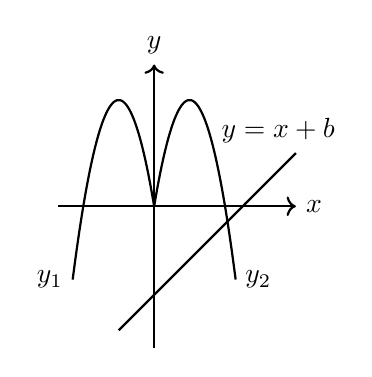
\begin{tikzpicture}[
                scale=0.45,
                declare function={
                    func(\x) = -3*(\x+1)^2 + 3;
                    func2(\x) = -3*(-\x+1)^2 + 3;
                    func3(\x) = \x -2.5;
                }
            ]
                \draw[->, thick] (-2.7, 0) -- (4, 0) node[right] {$x$};
                \draw[->, thick] (0, -4) -- (0, 4) node[above] {$y$};
            
                \draw[domain=-2.3:0, smooth, thick, variable=\x] plot ({\x}, {func(\x)});
                \pgfmathsetmacro{\xleft}{-2.3}
                \pgfmathsetmacro{\yleft}{func(\xleft)}
                % 在左侧端点右侧添加y₁标记
                \filldraw (\xleft,\yleft) circle (0pt);
                \node[left] at (\xleft,\yleft) {$y_1$};
            
                
                \draw[domain=0:2.3, smooth, thick, variable=\x] plot ({\x}, {func2(\x)});
                \pgfmathsetmacro{\xleft}{2.3}
                \pgfmathsetmacro{\yleft}{func2(\xleft)}
                % 在左侧端点右侧添加y₁标记
                \filldraw (\xleft,\yleft) circle (0pt);
                \node[right] at (\xleft,\yleft) {$y_2$};
                
                \draw[domain=-1:4, smooth, thick, variable=\x] plot ({\x}, {func3(\x)});
                \pgfmathsetmacro{\xleft}{3.5}
                \pgfmathsetmacro{\yleft}{func3(\xleft)+0.5}
                % 在左侧端点右侧添加y₁标记
                \filldraw (\xleft,\yleft) circle (0pt);
                \node[above] at (\xleft,\yleft) {$y=x+b$};
                
            \end{tikzpicture}
            例题图
        \end{center}
        \end{wrapfigure}

    \noindent
    \begin{example}
        
        如右图,函数 \( y_1 = -a(x+1)^2 + 3 \) (\( x < 0 \)) 的图象过原点,将其沿 \( y \) 轴翻折,得到函数 \( y_2 \) 的图象,把函数 \( y_1 \) 与 \( y_2 \) 的图象合并后称为函数 \( L \) 的图象.
        
        \begin{enumerate}
            \item \( a \) 的值为\underline{\hspace{3.5em}};函数 \( y_2 \) 的解析式为\underline{\hspace{3.5em}}(注明 \( x \) 的取值范围);
            \item 当直线 \( y = x + b \) 与函数 \( L \) 的图象有 3 个公共点时,求 \( b \) 的值.
        \end{enumerate}
        \begin{solution}
        
    \begin{enumerate}
    \item 分析:第一空求\(a\),观察解析式只有一个参数,所以只需要找出一个点就可以求\(y_1\)解析式和\(a\)的值,阅读题目得知\(y_1\)过原点即\((0,0)\),将\(x=0,y=0\)代入原解析式即可求出\(a\)的值,第二空求\(y_2\)的值,即求将\(y_1\)沿\(y\)轴翻折的解析式,只需改变\(y_1\)解析式的\(x\)为\(-x\)即可,最后注意标注自变量的取值范围.
    \item 分析:画草图分析(如右两小图),上下平移直线\(y=x+b\)发现只有两种情况与函数L有三个公共点,第一种:已知函数L过原点,当直线\(y=x+b\)也过原点(即\(b=0\)时),满足条件,第二种:直线\(y=x+b\)与函数L的\(y_2\)部分只有一个交点(即相切)的时候符合条件,此时要计算参数\(b\)的值需要结合前面学习抛物线交点相关问题的知识点,抓住直线与抛物线\(y_2\)只有一个交点这一条件,将二次函数\(y_2\)与一次函数\(y=x+b\)的解析式联立,得到一个含参数\(b\)的一元二次方程,因为只有一个交点所以该方程的判别式等于0,即\(\Delta=0\),依据判别式列出一个含参数\(b\)的方程,解方程就能得到第二种情况\(b\)的值.
    \end{enumerate}
    \end{solution}
    \end{example}
    \begin{wrapfigure}{r}{4cm}
    \subfigure[]{
    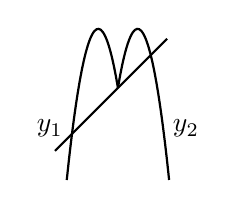
\begin{tikzpicture}[
            scale=0.25,
            declare function={
                func(\x) = -3*(\x+1)^2 + 3;
                func2(\x) = -3*(-\x+1)^2 + 3;
                func3(\x) = \x;
            }
        ]
            \draw[domain=-2.6:0, smooth, thick, variable=\x] plot ({\x}, {func(\x)});
            \pgfmathsetmacro{\xleft}{-2.3}
            \pgfmathsetmacro{\yleft}{func(\xleft)}
            % 在左侧端点右侧添加y₁标记
            \filldraw (\xleft,\yleft) circle (0pt);
            \node[left] at (\xleft,\yleft) {$y_1$};
        
            
            \draw[domain=0:2.6, smooth, thick, variable=\x] plot ({\x}, {func2(\x)});
            \pgfmathsetmacro{\xleft}{2.3}
            \pgfmathsetmacro{\yleft}{func2(\xleft)}
            % 在左侧端点右侧添加y₁标记
            \filldraw (\xleft,\yleft) circle (0pt);
            \node[right] at (\xleft,\yleft) {$y_2$};
            
            \draw[domain=-3.2:2.5, smooth, thick, variable=\x] plot ({\x}, {func3(\x)});
            
        \end{tikzpicture}
    }\subfigure[]{
    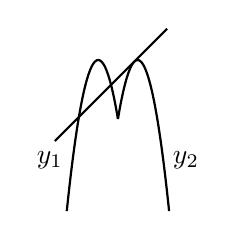
\begin{tikzpicture}[
            scale=0.25,
            declare function={
                func(\x) = -3*(\x+1)^2 + 3;
                func2(\x) = -3*(-\x+1)^2 + 3;
                func3(\x) = \x + 25/12;
            }
        ]
            \draw[domain=-2.6:0, smooth, thick, variable=\x] plot ({\x}, {func(\x)});
            \pgfmathsetmacro{\xleft}{-2.3}
            \pgfmathsetmacro{\yleft}{func(\xleft)}
            % 在左侧端点右侧添加y₁标记
            \filldraw (\xleft,\yleft) circle (0pt);
            \node[left] at (\xleft,\yleft) {$y_1$};
        
            
            \draw[domain=0:2.6, smooth, thick, variable=\x] plot ({\x}, {func2(\x)});
            \pgfmathsetmacro{\xleft}{2.3}
            \pgfmathsetmacro{\yleft}{func2(\xleft)}
            % 在左侧端点右侧添加y₁标记
            \filldraw (\xleft,\yleft) circle (0pt);
            \node[right] at (\xleft,\yleft) {$y_2$};
            
            \draw[domain=-3.2:2.5, smooth, thick, variable=\x] plot ({\x}, {func3(\x)});
            
        \end{tikzpicture}
    }
    
    \end{wrapfigure}
    
所以





\subsection{设参}
在学习一次函数时,我们就接触过设参,设参思想是处理二次函数综合问题的核心代数化策略,其本质是通过引入辅助变量(称为参数)将几何动态问题转化为可计算的代数模型。当抛物线上的点$P$位置变化时,设其横坐标为参数$t$,根据二次函数解析式 $y = ax^2 + bx + c$,点$P$的纵坐标可直接用含$t$的代数式表示为:
\[
y = at^2 + bt + c
\]
此时点$P$的完整坐标可记为:
\[
P(t,\  at^2 + bt + c)
\].该操作的数学意义在于:
\begin{enumerate}
    \item 将连续运动的点转化为连续变化的参数.
    \item 通过特定条件控制参数的取值,用于描述几何关系
\end{enumerate}
\begin{remark}
设参的前提是明确所求的目标,不要为了设参而设参    
\end{remark}


\begin{example}
如图\ref{fig:sp1},抛物线 \( y = -x^2 + 2x + 3 \) 与 \( x \) 轴交于 \( A \),\( B \) 两点,与 \( y \) 轴交于 \( C \) 点。
\begin{enumerate}
    \item 直接写出 \( A, B, C \) 点的坐标;  
    \item 过点 \( A \) 作两条直线分别交抛物线于第一象限点 \( P, Q \),交 \( y \) 轴于点 \( M, N, OM \cdot ON = n \)。当 \( n \) 为定值时,直线 \( PQ \) 是否必定经过某一定点?若经过,请你求出该定点坐标(用含 \( n \) 的式子表示);若不经过,请说明理由。
\end{enumerate}
\end{example}

\begin{wrapfigure}{r}{4cm}
    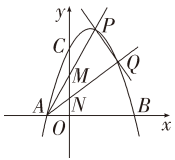
\includegraphics[width=1\linewidth]{figure/设参题1.png}
    \caption{}
    \label{fig:sp1}
\end{wrapfigure}

\begin{solution}
    分析:第一题:题目要求直接写出三个点的坐标,观察图像可以发现\(A,B\)两点是与\(x\)轴的交点,\(C\)点是与\(y\)轴的交点,题目给出了抛物线的一般式,能直接得出\(C\)点坐标为\((0,3\),观察解析式发现可以因式分解(十字相乘)将解析式写成交点式,即可得出\(A,B\)坐标为\(A(-1,0),B(3,0)\).
    
    第二题:题目实际上要求出直线\(PQ\)经过的定点,但是题目明显没有给出直线的解析式,此时就需要我们设出\(PQ\)的解析式为\(PQ:y=kx+m\) ,要求\(PQ\)先求\(P,Q\)两点,因为\(P,Q\)两点在抛物线上,也就是\(PQ\)与抛物线的两个交点,所以联立直线和抛物线得到\(kx+m=-x^2+2x+3\)整理可得\(x^2+(k-2)x+(m-3)\),由于过定点所以必定要消去\(m\)或者用代数式表示\(m\),因为题目要求用含\(n\)的代数式表达定点,所以\(m\)必定是一个含\(n\)的代数式,接下来尝试求\(m\),题目中给出的关于\(n\)的信息只有\(OM \cdot ON = n \),观察图像发现\(OM,ON\)实际上表示的是\(|y_M|\)和\(|y_N|\) 实际上是\(M,N\)两点的纵坐标,而这两点又是在两条直线\(PA,QA\)上,要想求\(M,N\)两点就得求直线\(PA,QA\),由上一题已知\(A(-1,0)\),还差\(P,Q\)的坐标才能分别求出两条直线\(PA,QA\)的解析式,而\(P,Q\)恰好在抛物线上,是抛物线与直线\(PQ\)的交点,就此我们建立了两个不同条件的关系(前面联立的方程就是抛物线与直线\(PQ\)的交点的方程),那么整理过的\(x^2+(k-2)x+(m-3)\)如何表达两个交点呢,显然可以运用韦达定理,两根之和等于二次项系数,两根之积等于常数项.
    
    此时设\(P(a,-a^2+2a+3),Q(b,-b^2+2b+3)\),根据韦达定理两根之和等于二次项系数,两根之积等于常数项,所以\(a+b=k-2, ab=m-3\),像要求\(M,N\)就需要求\(PA,QA\),现在已经设出\(P,Q\),因为两点确定一条直线,所以可以求出\(PA,QA\)的解析式分别为\(y=(3-a)(x+1),y=(3-a)(x+1)\),接下来就能求\(M,N\),因为\(M,N\)的横坐标都是0,所以代入求得\(M(0,a-3),N(0,b-3)\),所以\(OM=a-3,ON=b-3\),代入\( M, N, OM \cdot ON = n \),得\((a-3)(b-3)=n\),整理得\(ab-3(a+b)+9-n=0\),将\(a+b=k-2, ab=m-3\)代入该式得\(m=n-3k\),这样就达成了我们最初的目的,最后将\(m=n-3k\)代入\(PQ:y=kx+m\)就能得到\(PQ\)过定点$(3,n)$,注意写解前要先说:\(PQ\)过定点,再写过程.
\end{solution}

\subsection{二次函数与\textbf{线段}}

处理有关线段的问题,常常需要用到距离公式.

\begin{theorem}
设平面直角坐标系中两点 \( A(x_1,y_1) \) 和 \( B(x_2,y_2) \),则两点间距离 \( d \) 满足:
\[
d = \sqrt{(x_2 - x_1)^2 + (y_2 - y_1)^2}.
\]
\end{theorem}


\begin{wrapfigure}{r}{4cm}
    \begin{tikzpicture}[scale=0.7]
    % 坐标系
    \draw[->,thick] (-0.5,0) -- (5,0) node[right]{$x$};
    \draw[->,thick] (0,-0.5) -- (0,3) node[above]{$y$};
    
    % 标记点A和B
    \coordinate (A) at (1,1);
    \coordinate (B) at (3,2.5);
    \coordinate (C) at (3,1);
    
    % 绘制直角三角形
    \draw[thick] (A) -- (B) -- (C) -- cycle;
    \draw[dashed] (A) -- (C) node[midway,below]{$|x_2 - x_1|$};
    \draw[dashed] (B) -- (C) node[midway,right]{$|y_2 - y_1|$};
    
    % 标注点
    \filldraw (A) circle (1.5pt) node[below left]{$A(x_1,y_1)$};
    \filldraw (B) circle (1.5pt) node[above right]{$B(x_2,y_2)$};
    \filldraw (C) circle (1.5pt) node[below right]{$C(x_2,y_1)$};
    
    % 标注斜边
    \node at ($(A)!0.5!(B)$) [above=5pt] {$d$};
    \end{tikzpicture}
    \caption{距离公式证明}
\end{wrapfigure}
\begin{proof}



\begin{enumerate}
\item \textbf{构造直角三角形}:
过点 \( A \) 作水平线,过点 \( B \) 作垂直线,两线交于点 \( C(x_2,y_1) \),形成直角三角形 \( \triangle ABC \).

\item \textbf{确定直角边长度}:
\begin{align*}
\text{水平直角边 } AC &= |x_2 - x_1|,\\
\text{垂直直角边 } BC &= |y_2 - y_1|.
\end{align*}

\item \textbf{应用勾股定理}:
在 \( \triangle ABC \) 中,斜边 \( AB \) 满足:
\[
AB^2 = AC^2 + BC^2 = (x_2 - x_1)^2 + (y_2 - y_1)^2.
\]

\item \textbf{推导距离公式}:
两边取算术平方根(距离 \( d > 0 \))即得:
\[
d = \sqrt{(x_2 - x_1)^2 + (y_2 - y_1)^2}.\quad
\]
\end{enumerate}
\end{proof}
\begin{remark}
当两点在平行于坐标轴的直线上时,公式退化为绝对值形式(如 \( d = |x_1 - x_2| \)或\( d = |y_1 - x_2| \)).
\end{remark}

当前阶段有关线段的题目有求线段值、证明或运用线段关系、线段最值问题.学习本节需要具有良好的几何基础,本节主要以练习为主.

\subsubsection*{线段值}
\noindent
\begin{minipage}{1\linewidth}
    \begin{wrapfigure}{r}{3cm}
    \vspace{-2cm}
    \hspace{-1.4cm}
    \centering
    \begin{center}
    \centering
        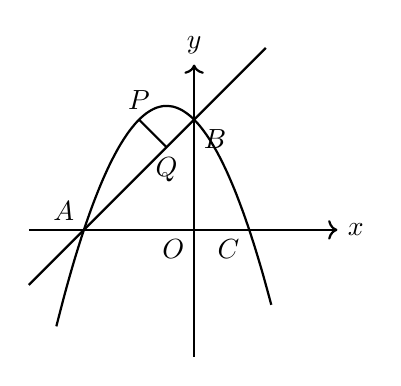
\begin{tikzpicture}[
            scale=0.7,
            declare function={
                func(\x) = -(\x+2)*(\x-1);
                func2(\x) = \x +2;
            }
        ]
            \draw[->, thick] (-3, 0) -- (2.6, 0) node[right] {$x$};
            \draw[->, thick] (0, -2.3) -- (0, 3) node[above] {$y$};

            \filldraw (-1,2) circle (0pt) node[above] {$P$};

            \filldraw (-2,0) circle (0pt) node[above left] {$A$};
            \filldraw (0,2) circle (0pt) node[below right] {$B$};
            \filldraw (1,0) circle (0pt) node[below left] {$C$};
            \filldraw (0,0) circle (0pt) node[below left] {$O$};
            \draw[black, thick] (-1,2) -- (-0.5,1.5) node[below] {$Q$};
        
            \draw[domain=-2.5:1.4, smooth, thick, variable=\x] plot ({\x}, {func(\x)});
            
            \draw[domain=-3:1.3, smooth, thick, variable=\x] plot ({\x}, {func2(\x)});
            
        \end{tikzpicture}
        例题图
        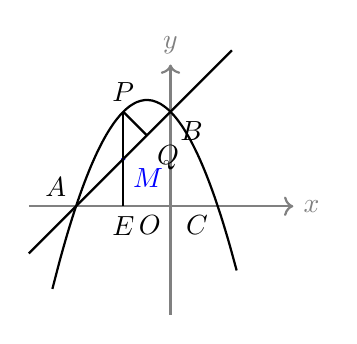
\begin{tikzpicture}[
            scale=0.6,
            declare function={
                func(\x) = -(\x+2)*(\x-1);
                func2(\x) = \x +2;
            }
        ]
            \draw[->, thick, gray] (-3, 0) -- (2.6, 0) node[right] {$x$};
            \draw[->, thick, gray] (0, -2.3) -- (0, 3) node[above] {$y$};

            \filldraw (-1,2) circle (0pt) node[above] {$P$};

            \filldraw (-2,0) circle (0pt) node[above left] {$A$};
            \filldraw (0,2) circle (0pt) node[below right] {$B$};
            \filldraw (1,0) circle (0pt) node[below left] {$C$};
            \filldraw (0,0) circle (0pt) node[below left] {$O$};
            \filldraw[blue] (-1,1) circle (1pt) node[below right, blue] {$M$};

            
            \draw[black, thick] (-1,2) -- (-0.5,1.5) node[below right] {$Q$};
            \draw[black, thick] (-1,2) -- (-1,0) node[below] {$E$};
            \draw[domain=-2.5:1.4, smooth, thick, variable=\x] plot ({\x}, {func(\x)});
            
            \draw[domain=-3:1.3, smooth, thick, variable=\x] plot ({\x}, {func2(\x)});
            
        \end{tikzpicture}
    \end{center}
    
    \end{wrapfigure}

    \begin{example}
        
        如图,在平面直角坐标系中,直线 \( y = x + 2 \) 与坐标轴交于 \( A \),\( B \) 两点,点 \( A \) 在 \( x \) 轴上,点 \( B \) 在 \( y \) 轴上,点 \( C \) 的坐标为(1,0),抛物线 \( y = -x^2-x + 2 \) 经过点 \( A \),\( B \),\( C \).若点 \( P \) 是抛物线上一动点,且在直线 \( AB \) 上方,过点 \( P \) 作 \( AB \) 的垂线段,垂足为点 \( Q \).当 \( PQ = \dfrac{\sqrt{2}}{2} \) 时,求点 \( P \) 的坐标.
        
    \end{example}

    \begin{solution}
    分析:由题可知\(PQ=\dfrac{\sqrt{2}}{2}\)和\(PQ\perp AB\)可以联想到需要想利用等腰直角三角形的边长比\(1:1:\sqrt{2}\),此时需要构造等腰直角三角形.就题目所给的条件来看无法构造两等边,所以考虑构造等角,由题意可知\(AO=OB,\angle AOB=90^\circ\),所以\(\triangle AOB\)是等腰直角三角形,所以\(\angle BAO=45^\circ\).由此可以做\(PE\perp x\)轴,易知\(\triangle AEM\)是等腰直角三角形,还可以知道\(\angle AEM=\angle PQM\),利用八字模型易知\(\triangle PQM\)是等腰直角三角形.构造等腰直角三角形完成.由三边比关系可以算出\(PM=1\)
    \par
    抓住\(PM=1\)这一条件,观察图像,发现\(PM=PE-ME=|y_P-y_M|=1\),可以设点\(P\)和点\(P\)的参数,代入该关系式,可以解出\(P\)横坐标,再讲\(P\)横坐标代回点\(P\)的纵坐标即可求出\(P\)的坐标
    \end{solution}

\end{minipage}

\subsubsection*{线段关系}
线段关系一般有数量关系,位置关系(垂直,平行),当提供线段关系等信息时需要运用几何的知识思考问题.
\begin{example}
如图\ref{fig:g1},已知抛物线 \( y = -x^2 + mx + 3 \) 与 \( x \) 轴交于 \( A, B \) 两点,与 \( y \) 轴交于点 \( C \),点 \( B \) 的坐标为 \((3,0)\).
\noindent
\begin{enumerate}
    \item 求抛物线的解析式;
    \item 若点 \( P \) 是直线 \( BC \) 上方抛物线上 的动点,过点 \( P \) 作直线 \( MN//y \) 轴,交 \( x \) 轴于点 \( N \),交直线 \( BC \) 于点 \( M \).设点 \( P \) 的横坐标为 \( t \),当 \( PN = 2PM \) 时,求点 \( P \) 的坐标.
\end{enumerate}
\begin{wrapfigure}{r}{7cm}
    \vspace{-1cm}
    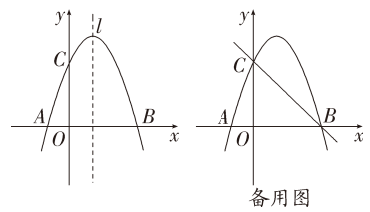
\includegraphics[width=1\linewidth]{figure/g1.png}
    \caption{}
    \label{fig:g1}
\end{wrapfigure}

\begin{solution}
    分析:(1)要求二次函数的解析式,题目给出的抛物线只有一个参数,又已知抛物线上点\(B(3,0)\),代入坐标即可求出解析式.得到解析式为\(y=-x^2+2x+3\)
    
    (2)画草图(如图\ref{fig:g2}),题目给出条件\( PN = 2PM \),所以需要先表示出\(P,M,N\)三点的坐标(\(P(t, -t^2+2t+3), M(t, -t+3), N(t, 0)\)),然后计算线段长,再代入关系式.得到关于\(t\)的一元二次方程\(t^2-4t+3=0\),解为\(t_1=1,t_2=3\),由于题目给\(P\)限定在第一象限,所以\(0<t<3\),舍去\(t=3\),最后再把\(t\)代入坐标得出结果\(P(1, 4)\)
\end{solution}

\end{example}

\begin{wrapfigure}{r}{3cm}
    \vspace{-1cm}
    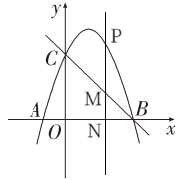
\includegraphics[width=1\linewidth]{figure/g2.png}
    \caption{}
    \label{fig:g2}
\end{wrapfigure}

\begin{remark}
着重掌握理解题目的能力
\end{remark}

\subsubsection*{线段最值}

在本阶段,求最值的方法主要有:两点之间线段最短、吹线段最短、三角形三边关系、将军饮马、配方求最值等.需要灵活分析题目,采用合适的方法.

\begin{example}
如图\ref{fig:g3},有抛物线\(y=-x^2-2x+3\).点$P$为抛物线第二象限上一个动点,过点$P$作$y$轴的平行线交$AC$于点$D$,\(A(-3,0), B(1, 0)\),求线段$PD$的最大值.

\begin{wrapfigure}{r}{3cm}
\vspace{-1cm}
    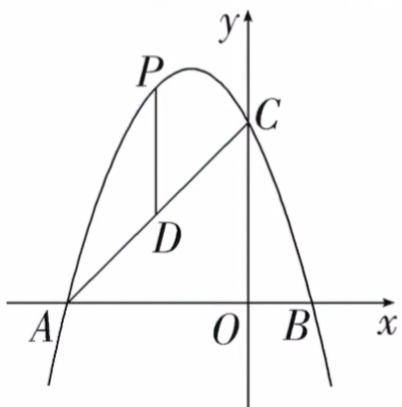
\includegraphics[width=1\linewidth]{figure/g3.png}
    \caption{}
    \label{fig:g3}
\end{wrapfigure}

\begin{solution}
    分析:由于要求线段\(PD\),所以先看点再看线,由题目可知\(P\)在抛物线上,\(D\)在直线\(AC\)上(求AC解析式得\(AC:y=x+3\)),题目给出了\(PD//y\)轴,证明\(P\)与\(D\)的横坐标相等,因此设点坐标可以得到两点\(P(m, -m^2-2m+3), D(m, m+3)\),再利用距离公式得到线段\(PD\)的长,此时得到一个二次多项式\(-m^2-3m\),对其配方,可以得到\(-(m-\dfrac{3}{2})^2+\dfrac{9}{4}\),所以当\(m=\dfrac{3}{2}\)时,该线段(多项式)取最大值,最大值为\(\dfrac{9}{4}\)
\end{solution}

\end{example}

\begin{wrapfigure}{l}{3cm}
    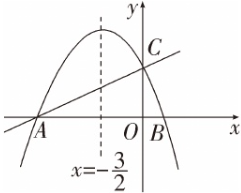
\includegraphics[width=1.2\linewidth]{figure/g4.png}
    \caption{}
    \label{fig:g4}
\end{wrapfigure}

\vspace{0.5cm}
\exas
{
如图,在平面直角坐标系中,直线 \( y = \dfrac{1}{2}x + 2 \) 与 \( x \) 轴交于点 \( A \),与 \( y \) 轴交于点 \( C \)。抛物线 \( y = ax^2 + bx + c \) 的对称轴是 \( x = -\dfrac{3}{2} \),且经过 \( A, C \) 两点,与 \( x \) 轴的另一交点为点 \( B \)。

\begin{enumerate}
    \item 求二次函数 \( y = ax^2 + bx + c \) 的解析式;
    \item 点 \( P \) 为线段 \( AB \) 上的动点,求 \( AP+2PC \) 的最小值
\end{enumerate}

}
{分析:
}




\subsection{二次函数与\textbf{面积}}

\subsubsection*{面积公式与割补}

\subsubsection*{铅锤法}

\subsubsection*{转化法}

\subsection{二次函数与\textbf{角度}}

\subsubsection*{角度定值或范围}

\subsubsection*{角度数量关系}

\subsection{二次函数与\textbf{特殊几何图形}}

\subsubsection*{特殊三角形}

\subsubsection*{特殊四边形}
%_______________________________________________________________________________________________________________________________________________
\chapter{旋转}

\section{旋转基本}

\subsection{旋转的性质}

我们把一个平面图形绕着平面内某一点\(O \)转动一个角度,叫做图形的旋转,点\(O \)叫做旋转中心,转动的角叫做旋转角 . 如果图形上的点\(P \)经过旋转变为点\(P' \),那么这两个点叫做这个旋转的对应点.

\begin{example}
    如下图,在\(Rt\triangle ABC \)中,\(\angle ABC = 90^\circ \),\(AB=BC=\sqrt{2}\),将\(\triangle ABC\)绕点\(C\)逆时针旋转\(60^\circ\),得到\(\triangle MNC\),连接\(BM\),则\(BM\)的长是 \underline{\hspace{3em}}
    
\begin{figure}[h]
    \raggedright
    \includegraphics[width=0.25\linewidth]{figure/example_rotation1.jpg}
    
    \label{fig:enter-label}
\end{figure}
    
\end{example}



\chapter{圆}





\section{圆基本}

平面内,到定点的距离等于定长的所有的点所组成的图形就是圆

定点:圆心

定长:半径

圆心决定圆的位置,半径决定圆的大小

同圆:圆心和半径都相等叫同圆
等圆:半径相等的叫等圆

弦:连接圆上两点的线段叫做弦

弧:圆上两点间的部分(本质是圆的一部分)

大于半圆的弧叫优弧,小于叫劣弧,等于半圆叫半圆

$\wideparen{AB}$

弦心距:弦到圆心的距离

圆心角:顶点在圆形的角

圆的任意部分弯曲程度始终相等

等弧:两个能完全重合的弧,必须在同圆或等圆中.

大小不一的圆弯曲程度不一

圆越大,弯曲程度(曲率)越小





---------------------------------




基本等量


同圆或等圆中一等得三等

弧

弦

圆心角

弦心距




\chapter*{后记}

\section*{建议}

建议在有实体人教教材配套使用.为了更加契合试题和方便理解,对部分章节的顺序做了调整,增加了一些章节.建议购买《初中5星学霸九年级数学RJ》和《实验班提优训练数学九年级上RMJY》,因为讲义中大部分题目来源于这两本书.由于讲义中的例题题目和解析比较近,建议自行遮住解析先做一遍例题.

\section*{勘误/修订日志}



\section*{声明}
部分例题和习题摘自《初中5星学霸九年级数学RJ》、《实验班提优训练数学九年级上RMJY》及部分来自互联网公开的免费资料

本讲义已经开源(地址:https://github.com/LanDiaoCha/Grade9-Maths-Lecture-Notes-PEP?tab=BSD-3-Clause-1-ov-file),请遵守协议内容,共同维护开源社区:禁止删除或修改原始版权声明和许可证文本、禁止未经许可使用版权所有者名称进行背书、禁止移除免责声明.
\par
BSD 3-Clause License

Copyright (c) 2025, 蓝调茶

Redistribution and use in source and binary forms, with or without
modification, are permitted provided that the following conditions are met:

1. Redistributions of source code must retain the above copyright notice, this
   list of conditions and the following disclaimer.

2. Redistributions in binary form must reproduce the above copyright notice,
   this list of conditions and the following disclaimer in the documentation
   and/or other materials provided with the distribution.

3. Neither the name of the copyright holder nor the names of its
   contributors may be used to endorse or promote products derived from
   this software without specific prior written permission.

THIS SOFTWARE IS PROVIDED BY THE COPYRIGHT HOLDERS AND CONTRIBUTORS "AS IS"
AND ANY EXPRESS OR IMPLIED WARRANTIES, INCLUDING, BUT NOT LIMITED TO, THE
IMPLIED WARRANTIES OF MERCHANTABILITY AND FITNESS FOR A PARTICULAR PURPOSE ARE
DISCLAIMED. IN NO EVENT SHALL THE COPYRIGHT HOLDER OR CONTRIBUTORS BE LIABLE
FOR ANY DIRECT, INDIRECT, INCIDENTAL, SPECIAL, EXEMPLARY, OR CONSEQUENTIAL
DAMAGES (INCLUDING, BUT NOT LIMITED TO, PROCUREMENT OF SUBSTITUTE GOODS OR
SERVICES; LOSS OF USE, DATA, OR PROFITS; OR BUSINESS INTERRUPTION) HOWEVER
CAUSED AND ON ANY THEORY OF LIABILITY, WHETHER IN CONTRACT, STRICT LIABILITY,
OR TORT (INCLUDING NEGLIGENCE OR OTHERWISE) ARISING IN ANY WAY OUT OF THE USE
OF THIS SOFTWARE, EVEN IF ADVISED OF THE POSSIBILITY OF SUCH DAMAGE.

\end{document}